\documentclass[12pt,letterpaper]{article}
\usepackage[T1]{fontenc}
\usepackage[letterpaper,margin=1in]{geometry}
\usepackage{amsmath,amssymb,amsthm,mathrsfs}
\IfFileExists{newtxtext.sty}{\usepackage{newtxtext,newtxmath}}{\usepackage{mathptmx}}
\usepackage{microtype,booktabs,enumitem,tikz}
\usepackage[hidelinks]{hyperref}
\numberwithin{equation}{section}
\allowdisplaybreaks[2]
\emergencystretch=2em
\newtheorem{theorem}{Theorem}[section]
\newtheorem{lemma}[theorem]{Lemma}
\newtheorem{proposition}[theorem]{Proposition}
\newtheorem{corollary}[theorem]{Corollary}
\theoremstyle{definition}
\newtheorem{definition}[theorem]{Definition}
\newtheorem{example}[theorem]{Example}
\theoremstyle{remark}
\newtheorem{remark}[theorem]{Remark}
\newtheorem{remarkyr}{Remark}
\renewcommand{\theremarkyr}{2026.\arabic{remarkyr}}
\newcommand{\OO}{\mathcal O_F}
\newcommand{\OEr}{\mathcal O_E}
\newcommand{\kk}{\mathbb F_q}
\newcommand{\Gt}{\widetilde G}
\newcommand{\cInd}{\operatorname{c-Ind}}
\newcommand{\tr}{\operatorname{tr}}
\newcommand{\val}{\operatorname{val}}
\newcommand{\diag}{\operatorname{diag}}
\newcommand{\Hom}{\operatorname{Hom}}
\newcommand{\Ext}{\operatorname{Ext}}
\newcommand{\Ad}{\operatorname{Ad}}
\newcommand{\Lie}{\operatorname{Lie}}
\newcommand{\BT}{\mathscr B}
\newcommand{\np}{n_{+}}
\newcommand{\nm}{n_{-}}
\newcommand{\sgn}{\epsilon}
\newcommand{\sm}[4]{\left(\begin{smallmatrix}#1&#2\\#3&#4\end{smallmatrix}\right)}
\title{Characters of supercuspidal representations of tame metaplectic covers of $\mathrm{SL}_2(F)$: a Bruhat--Tits tree approach\\[.5ex]\large Draft 1\\Merged, corrected and expanded version}
\author{David Joyner\thanks{This paper merges two sets of the first author's notes: notes of 1996 on the twofold cover, based on conversations with Jeff Adams and Jason Schultz, and notes of about 2000 on covers of odd degree. Their 2026 revisions are \cite{Jo26b} and \cite{Jo26a}. Email: \texttt{wdjoyner@gmail.com}.}, Gemini (Google), ChatGPT (OpenAI), and Claude (Anthropic)}
\date{Original notes: 1996 and 2000. Merged, corrected and expanded draft: 2026\\November 27, 2026}
\begin{document}
\maketitle
\begin{abstract}
This AI-aided paper used Gemini, ChatGPT and Claude to revise, correct and merge two sets of notes written in 1996 and about 2000. See the Acknowledgments for details. Let $F$ be a $p$-adic field with $p$ odd, and let $\Gt$ be a central cover of $G=\mathrm{SL}_2(F)$ by a cyclic group of order $n$ prime to $p$. We compare the characters of supercuspidal representations of $G$ and of genuine supercuspidal representations of $\Gt$ that are compactly induced from a maximal compact subgroup. The cover splits in exactly one way over the stabilizer of each vertex of the Bruhat--Tits tree. The character of a compactly induced representation at a regular elliptic element is a sum over the vertices fixed by the element, and for the cover each term is weighted by a ratio of two vertex splittings. We show that on regular elliptic elements these weights are governed by a single invariant of the cover, a sign $\sgn=\pm1$ that compares the two canonical lifts of $-I$. The genuine character equals the ordinary character up to the factor $\sgn$ raised to a power determined by the vertex types, and this factor occurs only near $-I$. The sign is $+1$ when $n$ is odd. For the Kubota cover defined by the $n$-th Hilbert symbol it is $-1$ exactly when $(q-1)/n$ is odd, where $q$ is the residue cardinality. For generic depth-zero supercuspidals we obtain closed formulas on the unramified elliptic tori. When $n$ is odd we deduce an $n$-th power character relation, and we show why no such relation exists for even $n$. The explicit formulas are restricted to depth zero and to unramified elliptic tori. The results for the split torus and for positive depth are partial.
\end{abstract}
\noindent\textbf{2020 MSC:} 22E50, 22E35, 20G05.\\
\textbf{Keywords:} metaplectic cover, tame central extension, Hilbert symbol, Bruhat--Tits tree, compact induction, depth-zero supercuspidal representation, character relations.
\tableofcontents

\section{Introduction}\label{sec:intro}
This section states the problem, the main results, the related literature and the notation.

The character of a representation induced from a compact open subgroup is a sum of traces, one for each conjugate of that subgroup containing the element. The conjugates of a maximal compact subgroup of $\mathrm{SL}_2(F)$ are the stabilizers of the vertices of a tree. So the sum runs over the vertices fixed by the element. We compare this sum term by term for a representation of $\mathrm{SL}_2(F)$ and for a genuine representation of a central cover. The cover splits over each vertex stabilizer in exactly one way. The central question is then geometric. Do the splittings attached to two different fixed vertices agree at the element being studied?

The two sets of notes merged here answered this question in two cases. For covers of odd degree the answer on elliptic elements is yes \cite{Jo26a}. For the twofold cover the answer is yes up to a sign that depends on the residue field \cite{Jo26b}. We show that both are instances of one statement, valid for every cover of degree prime to $p$. That statement also covers the even degrees $n\ge4$, which neither set of notes treated.

Throughout, $F$ is a finite extension of $\mathbb Q_p$ with $p$ odd. Its ring of integers is $\OO$, its uniformizer is $\varpi$, and its residue field is $\kk$ of order $q$. Write $G=\mathrm{SL}_2(F)$. A \emph{tame cover} of $G$ is a topological central extension
\begin{equation}\label{eq:cover}
 1\longrightarrow\mu_n\longrightarrow\Gt\xrightarrow{\ P\ }G\longrightarrow1
\end{equation}
by a cyclic group $\mu_n$ of order $n$ with $p\nmid n$ (Definition~\ref{def:tame}). We fix an injective character $\iota:\mu_n\to\mathbb C^\times$. A representation of $\Gt$ is \emph{genuine} if $\mu_n$ acts through $\iota$.

\begin{example}\label{ex:running}
The running example is $F=\mathbb Q_7$, with $q=7$. The Kubota covers of degree $n=2$, $3$ and $6$ are tame covers of $\mathrm{SL}_2(\mathbb Q_7)$ (Section~\ref{sec:kubota}). They will have signs $\sgn=-1$, $+1$ and $-1$.
\end{example}

\subsection*{Main results and their significance}
We describe the results in the order in which they are proved. The tree has two orbits of vertices under $G$, called types $0$ and $1$, with base vertices $v_0$ and $v_1$. Each vertex $v$ has a compact open stabilizer $K_v$.

\begin{enumerate}[leftmargin=2em]
\item \emph{Vertex splittings} (Proposition~\ref{prop:splittings}). For every tame cover and every vertex $v$ there is a unique homomorphism $s_v:K_v\to\Gt$ lifting the inclusion. No cocycle is needed. Uniqueness does not imply that $s_v$ and $s_{v'}$ agree on $K_v\cap K_{v'}$.
\item \emph{The central sign} (Definition~\ref{def:sign}, Proposition~\ref{prop:sign}). The element $-I$ fixes every vertex. The ratio $s_{v_1}(-I)s_{v_0}(-I)^{-1}$ lies in $\mu_n$ and has order at most two. Its image under $\iota$ is a sign $\sgn\in\{\pm1\}$ that depends only on the cover. If $n$ is odd then $\sgn=1$. For $z=\pm1$ write $\sgn(1)=1$ and $\sgn(-1)=\sgn$.
\item \emph{Weighted fixed-vertex formula} (Theorem~\ref{thm:weighted}). Let $\sigma_j$ be a representation of $K_{v_j}$, and let $\pi_j$ and $\widetilde\pi_j$ be the ordinary and genuine compact inductions. For a regular elliptic element $t$ fixing a vertex $w$, the character $\Theta_{\pi_j}(t)$ is a finite sum of local traces over the fixed vertices of type $j$. The genuine character $\Theta_{\widetilde\pi_j}(s_w(t))$ is the same sum with each term weighted by $\iota\bigl(s_w(t)s_v(t)^{-1}\bigr)$.
\item \emph{Direct comparison} (Theorem~\ref{thm:compare}). If $w$ has type $i$ and $t$ fixes an edge, then the reduction of $t$ has a repeated eigenvalue $z=\pm1$ and
\begin{equation}\label{eq:intro-main}
 \Theta_{\widetilde\pi_j}(s_w(t))=\sgn(z)^{j-i}\,\Theta_{\pi_j}(t).
\end{equation}
The factor is $-1$ exactly when $\sgn=-1$, $z=-1$ and $j\ne i$. If $t$ fixes only the vertex $w$, the two characters agree. This holds for inducing data of any depth, as long as both inductions are admissible.
\item \emph{Depth-zero formulas} (Theorem~\ref{thm:depthzero}, Corollary~\ref{cor:sum}). For the generic depth-zero types attached to a regular character $\theta$ of the finite nonsplit torus, and $t$ in an unramified elliptic torus at congruence depth $r\ge1$, the ordinary value is $\theta(z)\bigl((-1)^{r+1+j-i}q^r-1\bigr)$. The genuine value is this number times $\sgn(z)^{j-i}$. The terms of size $q^r$ cancel in the ordinary sum over $j$. In the genuine sum they cancel only after the factor $\sgn(z)^{j-i}$ is inserted.
\item \emph{The Kubota covers} (Propositions~\ref{prop:edge} and \ref{prop:apartment}, Corollary~\ref{cor:kubotasign}). For the cover defined by the $n$-th Hilbert symbol, the ratio of the two splittings on the Iwahori subgroup is the $n$-th power residue character of a diagonal entry. Hence $\sgn=-1$ exactly when $(q-1)/n$ is odd, that is, when $-1$ is not an $n$-th power in $\kk^\times$. For $n=2$ this is the condition $q\equiv3\pmod4$ of \cite{Jo26b}.
\item \emph{The power map} (Theorem~\ref{thm:power}). If $n$ is odd and prime to $q+1$, then $t\mapsto t^n$ is an automorphism of each unramified elliptic torus, and
\[
 \Theta_{\widetilde\pi_{j,\theta^{\langle n\rangle}}}\bigl(s_i(t^n)\bigr)=\Theta_{\pi_{j,\theta}}(t),
\]
where $\theta^{\langle n\rangle}$ is $\theta$ composed with the inverse of the $n$-th power map. If $n$ is even this map has kernel $\{\pm1\}$ on the torus, and no such reparameterization exists.
\item \emph{Split elements} (Proposition~\ref{prop:splitvanish}). The depth-zero characters of both kinds vanish at split elements with regular reduction.
\end{enumerate}

Table~\ref{tab:parity} summarizes how the parity of $n$ enters. The two rows that depend on parity have a common source. The sign $\sgn$ can be nontrivial only when $\mu_n$ contains an element of order two, and this is also the condition for $-1$ to lie in the kernel of the $n$-th power map.

\begin{table}[ht]
\centering
\caption{The role of the parity of the degree $n$. The last two rows assume that $F$ contains the $n$-th roots of unity, so that $n$ divides $q-1$.}\label{tab:parity}
\vspace{4pt}
\small
\begin{tabular}{@{}lll@{}}
\toprule
 & $n$ odd & $n$ even\\
\midrule
Central sign $\sgn$ & $+1$ & $\pm1$. Kubota cover: $-1$ iff $(q-1)/n$ is odd\\
Comparison \eqref{eq:intro-main} & no sign & sign $\sgn(z)^{j-i}$\\
$n$-th power map on an unramified torus & automorphism & kernel $\{\pm1\}$, image of index two\\
Reparameterization $\theta\mapsto\theta^{\langle n\rangle}$ & exists & does not exist\\
\bottomrule
\end{tabular}
\end{table}

\emph{Restrictions.} All results assume that $p$ is odd and that $p\nmid n$. The closed formulas of Section~\ref{sec:depthzero} are restricted to depth zero, to regular $\theta$ and to unramified elliptic tori. Section~\ref{sec:kubota} is restricted to the Kubota covers and assumes that $F$ contains the $n$-th roots of unity. Theorem~\ref{thm:power} is restricted to odd $n$. The ordinary character formulas for $\mathrm{SL}_2(F)$ are classical \cite{SS68}, and we claim no originality for them. Their derivation from the tree is included because the genuine formulas are obtained from the same sums.

\subsection*{Literature review}
The literature supplies the covers, the compact constructions and the character theory. We separate the work available when the original notes were written from later developments.

\subsubsection*{Through 2000}
Kubota \cite{Ku67} constructs covers of $\mathrm{SL}_2$ and $\mathrm{GL}_2$ over a local field from the norm residue symbol and gives the splitting over $\mathrm{SL}_2(\OO)$ when the degree is prime to $p$. Moore \cite{Mo68} and Matsumoto \cite{Ma69} extend the construction to general Steinberg symbols and to other groups. Gelbart \cite{Ge76} explains the Weil representation and the twofold cover, and extends the twofold cocycle to $\mathrm{GL}_2(F)$. Neukirch \cite{Ne86} supplies the local class field theory behind the Hilbert symbol. Kazhdan and Patterson \cite{KP84} use the compact splitting to study the unramified principal series and theta series on $n$-fold covers of $\mathrm{GL}_r(F)$.

Sally and Shalika \cite{SS68} compute the discrete-series characters of $\mathrm{SL}_2(F)$. Deligne and Lusztig \cite{DL76} construct the representations of finite reductive groups from characters of tori. For a supercuspidal representation realized by compact induction, the character on regular elliptic elements is a finite sum of Frobenius type. Sally \cite{Sa88} states this, and Kutzko \cite{Ku87} develops such sums for $\mathrm{GL}_\ell$ with $\ell$ prime. Moy and Prasad \cite{MP94,MP96} place the depth-zero constructions in a general framework based on the building. Manderscheid \cite{Ma84a,Ma84b} studies the supercuspidal representations of $\mathrm{SL}_2$ and of its twofold cover.

For the twofold cover, Waldspurger \cite{Wa80,Wa91} relates genuine representations to representations of $\mathrm{PGL}_2(F)$ through the theta correspondence. That is a different kind of comparison from the one studied here. For $n$-fold covers of $\mathrm{GL}_2(F)$ and $\mathrm{GL}_r(F)$, Flicker \cite{Fl80} and Flicker and Kazhdan \cite{FK86} use the trace formula to establish a correspondence with the linear group through an $n$-th power map on eigenvalues. Blondel \cite{Bl85} computes characters of supercuspidal representations of covers of $\mathrm{GL}_2$. The first author compares Hecke algebras of $\mathrm{SL}_2(F)$ and of its $n$-fold cover in \cite{Jo98}, and treats a supercuspidal correspondence for these covers in \cite{Jo99}. The present paper revisits the setting of \cite{Jo99} geometrically. It does not replace the full scope of that paper.

\subsubsection*{After 2000}
Howard and Weissman \cite{HW09} extend depth-zero theory to tame nonlinear covers. A key observation of theirs is that a pro-$p$ subgroup splits uniquely in a central extension whose kernel has order prime to $p$. Weissman \cite{We09} treats covers of tori, and Brylinski and Deligne \cite{BD01} classify the central extensions that come from algebraic $K$-theory. Li \cite{Li12} develops local harmonic analysis on covering groups, including the existence of character functions. Adams \cite{Ad03} studies character lifting for covers of $\mathrm{SL}(n)$. Manderscheid \cite{Ma04} describes Waldspurger's involution in terms of types.

On the linear side, Bonnaf\'e \cite{Bo11} and Digne and Michel \cite{DM20} give accounts of the characters of $\mathrm{SL}_2(\kk)$. Bushnell and Henniart \cite{BH06} treat compact induction and the character sums for $\mathrm{GL}_2$. Cunningham and Gordon \cite{CG09} prove depth-zero character formulas for $\mathrm{SL}_2$ on topologically unipotent elements. DeBacker and Spice \cite{DS18} study sums of characters of tame supercuspidal representations. Aubert and Plymen \cite{AP24} compare the Sally--Shalika formulas with endoscopic character identities for the depth-zero packets of $\mathrm{SL}_2$. Casselman's notes \cite{Ca14} describe the tree. The two manuscripts merged here are \cite{Jo26a}, for odd degree, and \cite{Jo26b}, for the twofold cover.

\begin{example}
The finite nonsplit torus over $\mathbb F_7$ is cyclic of order eight. Cubing permutes it. Squaring does not, since its image has four elements. This is the reason for the last two rows of Table~\ref{tab:parity} in the running example.
\end{example}

\subsection*{Notation}
The following notation is used throughout. In the running example $\OO=\mathbb Z_7$ and $\varpi=7$.
\begin{center}
\small
\begin{tabular}{@{}lp{.70\textwidth}@{}}
\toprule
Symbol & Meaning\\ \midrule
$F,\OO,\varpi,\kk,q,p$ & Local field, integers, uniformizer, residue field of odd order $q$ and characteristic $p$\\
$G,\Gt,P$ & $\mathrm{SL}_2(F)$, a tame cover, the covering projection\\
$\mu_n,\iota$ & The kernel of $P$, cyclic of order $n$ with $p\nmid n$, and an injective character of it\\
$\BT,v_0,v_1,D$ & Bruhat--Tits tree, the adjacent base vertices, $D=\diag(\varpi,1)$ with $v_1=Dv_0$\\
$B^t$, $B(v,r)$ & Set of vertices fixed by $t$, ball of radius $r$ around $v$\\
$K_v,K_v^+,s_v$ & Vertex stabilizer, its pro-$p$ radical, its unique splitting\\
$K_i,s_i$ & $K_{v_i}$ and $s_{v_i}$ for $i=0,1$\\
$I,I^+$ & Stabilizer of the base edge and its pro-$p$ radical\\
$\lambda_{v\to v'}(k)$ & Residue eigenvalue of $k$ on the oriented edge from $v$ to $v'$\\
$c_{w,v}(k)$ & The element $s_w(k)s_v(k)^{-1}$ of $\mu_n$\\
$\sgn$, $\sgn(z)$ & Central sign of the cover, with $\sgn(1)=1$ and $\sgn(-1)=\sgn$\\
$T_i,\bar T$ & Unramified norm-one torus at $v_i$ and its finite reduction\\
$\theta,\sigma_\theta,\chi_\theta$ & Regular character of $\bar T$, cuspidal representation, its character\\
$\theta^{\langle n\rangle}$ & The character $\bar\tau\mapsto\theta(\bar\tau^{e})$, where $en\equiv1\pmod{q+1}$\\
$\pi_j,\widetilde\pi_j$ & Ordinary and genuine compact inductions from type $j$\\
$\Theta_\pi$ & Character function of $\pi$\\
$(a,b)_n,\ \omega$ & $n$-th Hilbert symbol of $F$, $n$-th power residue character of $\kk^\times$\\
$\ell$ & Quadratic character of $\kk^\times$, equal to $\omega$ when $n=2$\\
$\beta$, $x(g)$ & Kubota cocycle and the function used to define it\\
$\np(x),\nm(x)$ & Upper and lower elementary unipotent matrices\\
$h(u),w(t)$ & $\diag(u,u^{-1})$ and $\np(t)\nm(-t^{-1})\np(t)$\\
\bottomrule
\end{tabular}
\end{center}

\section{Background: the tree, compact induction and characters}\label{sec:background}
This section recalls the geometry of the tree and the representation theory used later. It also proves the elementary lemmas that carry the geometric part of the argument. Nothing in this section involves a cover. The running example is the tree of valency eight over $\mathbb Q_7$.

\subsection*{Lattices, vertices and edges}
We describe the tree by lattices, since the reduction of a group element at a vertex is then visible.

A \emph{lattice} is the $\OO$-span of an $F$-basis of $F^2$. The vertices of $\BT$ are the homothety classes $[L]$, where $L$ and $aL$ are identified for $a\in F^\times$. Two vertices are adjacent if they have representatives with $\varpi L\subsetneq L'\subsetneq L$. The neighbors of $[L]$ correspond to the lines in $L/\varpi L\cong\kk^2$, so there are $q+1$ of them. The resulting graph is a tree \cite{Ca14}. Distance is computed by elementary divisors. If $L'=\OO\varpi^a e_1+\OO\varpi^b e_2$ for a basis $e_1,e_2$ of $L$, then $d([L],[L'])=|a-b|$.

Let $v_0=[\OO^2]$, $D=\diag(\varpi,1)$ and $v_1=Dv_0$. The parity of the distance from $v_0$ to $[L]$ equals the parity of the valuation of the determinant of a basis of $L$. An element of $G$ has determinant one, so it preserves this parity. Hence there are at least two $G$-orbits of vertices. There are exactly two, $Gv_0$ and $Gv_1$. To see this, take a matrix $g\in\mathrm{GL}_2(F)$ carrying $\OO^2$ to a lattice of even type. Multiply by a scalar to make $\det g$ a unit, and then replace $g$ by $g\,\diag(1,\det g^{-1})$, which carries $\OO^2$ to the same lattice. The same argument applies to $v_1$. We say that a vertex in $Gv_i$ has \emph{type} $i$. Adjacent vertices have different types.

The stabilizer $K_v$ of a vertex $v=[L]$ in $G$ is the stabilizer of the lattice $L$. Indeed, if $gL=aL$ then $\det g=1$ forces $\val(a)=0$. The base stabilizers are
\begin{equation}\label{eq:ki}
 K_0=\mathrm{SL}_2(\OO),\qquad K_1=DK_0D^{-1}
 =\Bigl\{\sm{a}{\varpi b}{\varpi^{-1}c}{d}:\sm abcd\in K_0\Bigr\}.
\end{equation}
The group $K_v$ acts on $L/\varpi L$ with determinant one. This action is the \emph{reduction at $v$}. Its kernel $K_v^+$ is a pro-$p$ group, and $K_v/K_v^+\cong\mathrm{SL}_2(\kk)$. The groups $K_0$ and $K_1$ represent the two conjugacy classes of maximal compact subgroups of $G$.

\begin{figure}[ht]
\centering
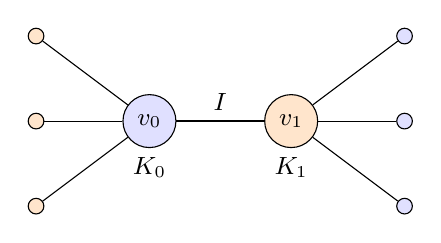
\begin{tikzpicture}[scale=.9, every node/.style={font=\small}]
\node[circle,draw,fill=blue!12] (a) at (0,0) {$v_0$};
\node[circle,draw,fill=orange!20] (b) at (2,0) {$v_1$};
\draw[thick] (a)--node[above] {$I$} (b);
\foreach \y in {-1.2,0,1.2}{
\node[circle,draw,fill=orange!20,inner sep=2pt] (l) at (-1.6,\y) {};
\draw (a)--(l);
\node[circle,draw,fill=blue!12,inner sep=2pt] (r) at (3.6,\y) {};
\draw (b)--(r);}
\node at (0,-.65) {$K_0$};
\node at (2,-.65) {$K_1$};
\end{tikzpicture}
\caption{Two adjacent vertex types and their edge stabilizer. The other branches are schematic.}
\label{fig:edge}
\end{figure}

The next lemma attaches a residue eigenvalue to an element fixing an oriented edge.

\begin{lemma}[Reduction on an edge]\label{lem:edgered}
Let $v=[L]$ and $v'=[L']$ be adjacent with $\varpi L\subsetneq L'\subsetneq L$, and let $k\in K_v\cap K_{v'}$. Then $k$ acts on the one-dimensional space $L/L'$ by a scalar $\lambda\in\kk^\times$ and on the line $L'/\varpi L$ by $\lambda^{-1}$. The reductions of $k$ at $v$ and at $v'$ are both triangularizable with eigenvalues $\lambda,\lambda^{-1}$.
\end{lemma}
\begin{proof}
We have $kL=L$ and $kL'=L'$, so the reduction of $k$ at $v$ preserves the line $L'/\varpi L$ of $L/\varpi L$. The action on $L/\varpi L$ has determinant one, so the scalars on the line and on the quotient $L/L'$ are inverse to each other. At $v'$, the space $L'/\varpi L'$ contains the line $\varpi L/\varpi L'$. Multiplication by $\varpi$ commutes with $k$ and identifies $L/L'$ with this line, so $k$ acts on it by $\lambda$. The quotient is $L'/\varpi L$, on which $k$ acts by $\lambda^{-1}$.
\end{proof}

We write $\lambda_{v\to v'}(k)$ for the scalar by which $k$ acts on $L/L'$. It does not depend on the choice of the pair $L\supsetneq L'$, since any other choice is a common multiple. Applying the lemma to the pair $L'\supsetneq\varpi L$ gives
\begin{equation}\label{eq:lambda-inv}
 \lambda_{v'\to v}(k)=\lambda_{v\to v'}(k)^{-1}.
\end{equation}
The map $k\mapsto\lambda_{v\to v'}(k)$ is a homomorphism from the edge stabilizer $I_e=K_v\cap K_{v'}$ to $\kk^\times$. Its kernel $I_e^+$ consists of the elements of $I_e$ whose reductions at $v$ and at $v'$ are unipotent. This kernel contains $K_v^+$ with a quotient of order $q$, so it is a pro-$p$ group. For $g\in G$ we have $\lambda_{gv\to gv'}(gkg^{-1})=\lambda_{v\to v'}(k)$.

\begin{example}\label{ex:baseedge}
The base edge joins $v_0=[\OO^2]$ and $v_1=[\varpi\OO\oplus\OO]$. By \eqref{eq:ki}, its stabilizer $I=K_0\cap K_1$ consists of the matrices $\sm abcd\in K_0$ with $b\in\varpi\OO$. Here $L/L'$ is spanned by the image of the first basis vector, so $\lambda_{v_0\to v_1}(k)=\bar a$. The group $I^+$ is the set of $k\in I$ with $a\equiv d\equiv1$ modulo $\varpi$, and $I/I^+\cong\kk^\times$ by $k\mapsto\bar a$. Every $k\in I$ lies in $h(a)I^+$, where $h(a)=\diag(a,a^{-1})$. Also, $D^mv_0=[\varpi^m\OO\oplus\OO]$ lies at distance $|m|$ from $v_0$, and $\diag(\varpi,\varpi^{-1})$ translates this line of vertices by two edges. For a unit $u$ the element $h(u)$ fixes every vertex of this line, and $\lambda_{D^mv_0\to D^{m+1}v_0}(h(u))=\bar u$ for every integer $m$.
\end{example}

\subsection*{Fixed vertices of elliptic elements}
The character formulas are sums over fixed vertices. We show that for a regular elliptic element this set is finite, nonempty and connected, and we find the residue eigenvalues on its edges.

An element $t\in G$ is \emph{regular elliptic} if its characteristic polynomial is irreducible over $F$. Write $B^t$ for the set of vertices fixed by $t$.

\begin{lemma}[Fixed sets]\label{lem:fixedset}
Let $t\in G$ be regular elliptic. Then $B^t$ is nonempty and finite. For any $x\in G$, the set $B^x$ is connected: the geodesic between two fixed vertices consists of fixed vertices.
\end{lemma}
\begin{proof}
Let $E=F[t]$, a quadratic field extension of $F$. Choose a nonzero vector $e\in F^2$. The map $y\mapsto ye$ identifies $E$ with $F^2$, and $t$ acts as multiplication by an element $\tau\in E$ with norm $\det t=1$. Hence $\tau\in\OEr^\times$, and the lattice $\OEr$ is fixed. So $B^t$ is nonempty.

A lattice $L\subset E$ satisfies $tL=L$ if and only if it is a module over the ring $\OO[\tau]$. Here we use that $t^{-1}=\tr(t)-t$ lies in $\OO[\tau]$. The ring $\OO[\tau]$ is an $\OO$-lattice in $E$ contained in $\OEr$, so $\varpi^r\OEr\subset\OO[\tau]$ for some $r\ge0$. Let $L$ be such a module and put $M=\OEr L$. Then $M$ is a fractional ideal of $E$ and
\[
 \varpi^rM=\varpi^r\OEr L\subset\OO[\tau]L=L\subset M .
\]
After scaling $L$ by a power of $\varpi$ we may assume that $M$ is $\OEr$ or the maximal ideal of $\OEr$. For each of these two choices there are finitely many lattices between $\varpi^rM$ and $M$. So $B^t$ is finite.

For the last statement, $x$ acts on $\BT$ as an automorphism. It maps the geodesic between two fixed vertices to a geodesic with the same endpoints. Geodesics in a tree are unique, so this geodesic is fixed pointwise.
\end{proof}

\begin{lemma}[Repeated residue eigenvalue]\label{lem:repeated}
Let $t$ be regular elliptic and suppose that $t$ fixes an edge. Then there is a sign $z=\pm1$ such that the reduction of $t$ at every fixed vertex has characteristic polynomial $(X-z)^2$. For every edge $e=\{v,v'\}$ fixed by $t$ we have $\lambda_{v\to v'}(t)=z$, and $t\in zI\cdot I_e^+$.
\end{lemma}
\begin{proof}
Let $v=[L]$ be a fixed vertex. The characteristic polynomial of $t$ on $L$ is that of $t$ on $F^2$. It has coefficients in $\OO$, and its reduction $\bar\chi$ is the characteristic polynomial of the reduction of $t$ at $v$. So $\bar\chi$ is the same at all fixed vertices. By Lemma~\ref{lem:edgered} its roots are $\lambda^{\pm1}$ with $\lambda=\lambda_{v\to v'}(t)\in\kk^\times$. If these were distinct, Hensel's lemma would lift them to roots in $F$, contradicting ellipticity. So $\lambda=\lambda^{-1}$, which gives $\lambda=z=\pm1$ and $\bar\chi=(X-z)^2$. The element $zI$ is central and fixes every vertex, and $\lambda_{v\to v'}(zI)=z$. So $zt$ lies in the kernel $I_e^+$ of $\lambda_{v\to v'}$.
\end{proof}

\begin{example}
A split element behaves differently. The matrix $h(3)=\diag(3,3^{-1})$ over $\mathbb Q_7$ fixes every vertex $D^mv_0$, so its fixed set is infinite. Its residue eigenvalue on each of these edges is $3^{\pm1}$, which is not $\pm1$. Its characteristic polynomial is reducible.
\end{example}

\subsection*{Compact induction and the vertex model}
We recall compact induction and decompose its space into pieces indexed by vertices.

Let $H$ be a compact open subgroup of $G$ and $\sigma$ a finite-dimensional smooth representation of $H$ on $V_\sigma$. The \emph{compact induction} $\cInd_H^G\sigma$ is the space of functions $f:G\to V_\sigma$ with $f(hg)=\sigma(h)f(g)$ whose support is a finite union of cosets $Hg$. The group acts by right translation, $(\pi(x)f)(y)=f(yx)$. The same definition applies to a cover of $G$ and to an open subgroup of it with compact image in $G$.

Fix $j\in\{0,1\}$ and a representation $\sigma_j$ of $K_j$. For a vertex $v=gv_j$ of type $j$ define a representation of $K_v=gK_jg^{-1}$ by $\sigma_v(k)=\sigma_j(g^{-1}kg)$. Its isomorphism class, and so its trace, does not depend on the choice of $g$.

\begin{lemma}[Vertex model]\label{lem:model}
Let $\pi_j=\cInd_{K_j}^G\sigma_j$ act on $V$. For $v=gv_j$ let $V_v\subset V$ be the subspace of functions supported on $K_jg^{-1}$. Then $V=\bigoplus_{v\in Gv_j}V_v$ and $\pi_j(x)V_v=V_{xv}$ for $x\in G$. The representation of $K_v$ on $V_v$ is isomorphic to $\sigma_v$.
\end{lemma}
\begin{proof}
The coset $K_jg^{-1}$ depends only on $v$, and distinct vertices give disjoint cosets. This gives the direct sum. If $f$ is supported on $K_jg^{-1}$, then $\pi_j(x)f$ is supported on $K_jg^{-1}x^{-1}=K_j(xg)^{-1}$. Evaluation $f\mapsto f(g^{-1})$ is a linear isomorphism $V_v\to V_{\sigma_j}$. For $k=gk'g^{-1}\in K_v$ we get $(\pi_j(k)f)(g^{-1})=f(k'g^{-1})=\sigma_j(k')f(g^{-1})$.
\end{proof}

\begin{example}
Inflate a cuspidal representation of $\mathrm{SL}_2(\mathbb F_7)$ of dimension six along $K_0\to\mathrm{SL}_2(\mathbb F_7)$ and compactly induce to $G$. Each $V_v$ has dimension six, and there is one for each vertex of type $0$. The induced space is infinite-dimensional.
\end{example}

\subsection*{Admissibility and characters}
We recall how a character is attached to an infinite-dimensional representation and express it through the vertex model.

A smooth representation is \emph{admissible} if its invariants under every compact open subgroup are finite-dimensional. A \emph{supercuspidal} representation is an irreducible admissible representation that is not a subquotient of a representation parabolically induced from a proper parabolic subgroup. Fix a Haar measure on $G$. For a locally constant compactly supported function $f$ on $G$ put $\pi(f)=\int_Gf(g)\pi(g)\,dg$. If $\pi$ is admissible, then $\pi(f)$ has finite rank and $f\mapsto\tr\pi(f)$ is the \emph{distribution character}. Suppose that on an open set $U$ there is a locally constant function $\Theta_\pi$ with $\tr\pi(f)=\int_Uf(g)\Theta_\pi(g)\,dg$ for all $f$ supported in $U$. Then $\Theta_\pi$ is unique, and we call it the \emph{character function} of $\pi$ on $U$. Harish-Chandra proved that such a function exists on the regular semisimple set, and Li \cite{Li12} proved the analogue for covering groups. We do not need these theorems on the sets studied below, because the function is exhibited directly.

\begin{lemma}[Block traces]\label{lem:blocks}
Assume that $\pi_j=\cInd_{K_j}^G\sigma_j$ is admissible. Then for every locally constant compactly supported $f$,
\begin{equation}\label{eq:blocks}
 \tr\pi_j(f)=\sum_{v\in Gv_j}\int_{K_v}f(g)\,\tr\sigma_v(g)\,dg ,
\end{equation}
and only finitely many terms are nonzero.
\end{lemma}
\begin{proof}
The operator $T=\pi_j(f)$ has finite rank. Its image lies in $W=\bigoplus_{v\in S}V_v$ for a finite set $S$ of vertices. The trace of $T$ equals the trace of its restriction to $W$, which is the sum over $v\in S$ of the traces of the diagonal blocks $P_vT|_{V_v}$. Here $P_v$ is the projection onto $V_v$. For $v\notin S$ the block is zero. Let $\varphi\in V_v$. By Lemma~\ref{lem:model}, $\pi_j(g)\varphi$ lies in $V_{gv}$. Its component in $V_v$ is $\pi_j(g)\varphi$ if $g\in K_v$ and zero otherwise. The integral defining $T\varphi$ is a finite sum, so $P_vT\varphi=\int_{K_v}f(g)\pi_j(g)\varphi\,dg$. Taking traces and using Lemma~\ref{lem:model} gives \eqref{eq:blocks}.
\end{proof}

\begin{example}\label{ex:nonadm}
Let $\sigma_0$ be the trivial representation of $K_0$. Then $\pi_0$ is the space of finitely supported functions on the vertices of type $0$, and $\tr\sigma_v(t)=1$ for every fixed vertex. This $\pi_0$ is not admissible. The indicator functions of the orbits of $K_0$ on these vertices are infinitely many linearly independent $K_0$-invariant vectors. The hypothesis of admissibility is a real restriction on $\sigma_j$.
\end{example}

\subsection*{Unramified elliptic tori}
The explicit formulas of Section~\ref{sec:depthzero} concern the following tori.

Let $E/F$ be the unramified quadratic extension. Identify $F^2$ with $E$ by an $\OO$-basis of $\OEr$. Multiplication embeds the norm-one group $E^1$ into $K_0$, and we call the image $T_0$. Set $T_1=DT_0D^{-1}\subset K_1$. Every element of $T_i$ other than $\pm I$ is regular elliptic. Reduction at $v_i$ maps $T_i$ onto the cyclic group $\bar T=\ker(N_{\mathbb F_{q^2}/\kk})$ of order $q+1$, and the kernel of this map is a pro-$p$ group. The tori $T_0$ and $T_1$ are conjugate in $\mathrm{GL}_2(F)$ and not in $G$. Indeed, the normalizer of $T_0$ in $\mathrm{GL}_2(F)$ is generated by $E^\times$ and the Galois conjugation of $E$. The determinants of its elements are norms from $E^\times$ up to sign, so they have even valuation. If $gT_0g^{-1}=T_1$ with $g\in G$, then $D^{-1}g$ would lie in this normalizer and have determinant $\varpi^{-1}$. Thus $T_0$ and $T_1$ represent the two conjugacy classes in the stable class of unramified elliptic tori of $G$.

\begin{example}\label{ex:torus}
Over $\mathbb Q_7$ the number $3$ is not a square modulo $7$, so $E=\mathbb Q_7(\sqrt3)$. The norm-one group consists of the $\alpha+\beta\sqrt3$ with $\alpha^2-3\beta^2=1$. In the basis $(1,\sqrt3)$ such an element acts by the matrix $\sm{\alpha}{3\beta}{\beta}{\alpha}$. Here $\bar T$ has order eight.
\end{example}

\section{Tame covers and vertex splittings}\label{sec:cover}
This section defines the covers, proves that each vertex stabilizer has exactly one splitting, and isolates the invariant that measures the disagreement of two splittings at $-I$. No cocycle is used. Explicit cocycles enter only in Section~\ref{sec:kubota}.

\subsection*{Tame covers and genuine representations}
We fix the class of covers and the convention for genuine representations.

\begin{definition}\label{def:tame}
A \emph{tame cover} of $G=\mathrm{SL}_2(F)$ is a topological group $\Gt$ with a continuous surjective homomorphism $P:\Gt\to G$ that is a local homeomorphism and whose kernel is a central cyclic subgroup of order $n$, where $p\nmid n$. We write $\mu_n$ for the kernel. A \emph{splitting} over a subgroup $H\subset G$ is a homomorphism $s:H\to\Gt$ with $P\circ s=\mathrm{id}_H$.
\end{definition}

The group $\Gt$ is locally compact and totally disconnected, because $G$ is and $P$ is a local homeomorphism. The preimage of a compact open subgroup of $G$ is a compact open subgroup of $\Gt$, so it is a profinite group. Fix an injective character $\iota:\mu_n\to\mathbb C^\times$. A representation $\widetilde\pi$ of $\Gt$ is \emph{genuine} if $\widetilde\pi(\zeta)=\iota(\zeta)$ for $\zeta\in\mu_n$. A genuine representation does not factor through $G$ unless $n=1$. Its character function satisfies $\Theta_{\widetilde\pi}(\zeta\widetilde g)=\iota(\zeta)\Theta_{\widetilde\pi}(\widetilde g)$.

\begin{example}\label{ex:covers}
The product $G\times\mu_n$ is a tame cover, with the splitting $g\mapsto(g,1)$ over all of $G$. The Kubota cover of Section~\ref{sec:kubota} is the set $G\times\mu_n$ with a multiplication twisted by the $n$-th Hilbert symbol. It exists when $F$ contains the $n$-th roots of unity. Over $\mathbb Q_7$ this allows $n=2,3,6$. By a theorem of Moore \cite{Mo68} the topological central extensions of $\mathrm{SL}_2(F)$ are classified by the roots of unity of $F$. We recall this for orientation and do not use it.
\end{example}

\subsection*{Existence and uniqueness of vertex splittings}
We show that a tame cover splits over each vertex stabilizer and that the splitting is unique. Uniqueness uses generation by unipotent elements. Existence uses the vanishing of a cohomology group of the finite group $\mathrm{SL}_2(\kk)$.

Write $\np(x)=\sm1x01$ and $\nm(x)=\sm10x1$ for $x\in F$. For $t\in F^\times$ put
\[
 w(t)=\np(t)\,\nm(-t^{-1})\,\np(t)=\sm{0}{t}{-t^{-1}}{0},
 \qquad h(t)=\diag(t,t^{-1})=w(t)w(1)^{-1}.
\]
For $k=\sm abcd\in K_0$ one has the factorizations
\begin{equation}\label{eq:word}
 k=\np\!\Bigl(\frac{a-1}{c}\Bigr)\nm(c)\,\np\!\Bigl(\frac{d-1}{c}\Bigr)\ \ (c\in\OO^\times),
 \qquad
 k=\nm\!\Bigl(\frac ca\Bigr)h(a)\,\np\!\Bigl(\frac ba\Bigr)\ \ (c\in\varpi\OO),
\end{equation}
with all arguments in $\OO$ and $a\in\OO^\times$ in the second case. Since $h(a)=w(a)w(1)^{-1}$ is a product of unipotent elements of $K_0$, the group $K_0$ is generated by its upper and lower unipotent elements. The same holds for $K_1=DK_0D^{-1}$, because conjugation by $D$ preserves the upper and the lower unipotent subgroups.

We use one elementary fact repeatedly. Let $U$ be a pro-$p$ group and let $\chi:U\to\mu_n$ be a homomorphism, not assumed continuous. Then $\chi$ is trivial. Indeed, the closed subgroup generated by an element $x\in U$ is a quotient of $\mathbb Z_p$, on which multiplication by $n$ is bijective. So $x=y^n$ for some $y\in U$, and $\chi(x)=\chi(y)^n=1$.

\begin{proposition}[Vertex splittings]\label{prop:splittings}
Let $\Gt$ be a tame cover. For every vertex $v$ there is a unique splitting $s_v:K_v\to\Gt$. It is continuous, and $P^{-1}(K_v)=\mu_n\times s_v(K_v)$. For $g\in G$, any lift $\widetilde g\in P^{-1}(g)$ and $k\in K_v$,
\begin{equation}\label{eq:equiv}
 s_{gv}(gkg^{-1})=\widetilde g\,s_v(k)\,\widetilde g^{-1}.
\end{equation}
\end{proposition}
\begin{proof}
\emph{Uniqueness.} Two splittings over $K_v$ differ by a homomorphism $\chi:K_v\to\mu_n$. The group $K_v$ is conjugate in $G$ to $K_0$ or $K_1$, so it is generated by unipotent elements. Each unipotent element $x$ of $K_v$ lies in $U\cap K_v$ for a unipotent subgroup $U\cong F$ of $G$. This intersection is a compact subgroup of $F$, hence a pro-$p$ group. So $\chi(x)=1$ by the fact above, and $\chi$ is trivial.

\emph{Existence.} Put $E=P^{-1}(K_v)$ and $E^+=P^{-1}(K_v^+)$. These are profinite groups. Every finite quotient of $E^+$ is a central extension of a $p$-group by a quotient of $\mu_n$. Such a finite group is nilpotent, and it is the direct product of its Sylow $p$-subgroup and the image of $\mu_n$. Passing to the limit, $E^+=\mu_n\times S$, where $S$ is the unique maximal pro-$p$ subgroup of $E^+$. This is the observation of \cite[Prop.~2.3]{HW09}. The subgroup $S$ is preserved by every topological automorphism of $E^+$, so it is normal in $E$. The quotient $\bar E=E/S$ is a finite group, and it is a central extension of $K_v/K_v^+\cong\mathrm{SL}_2(\kk)$ by $\mu_n$.

We claim that $H^2(\mathrm{SL}_2(\kk),\mu_n)=0$, with trivial action on $\mu_n$. Write $\Gamma=\mathrm{SL}_2(\kk)$. By the universal coefficient theorem,
\[
 H^2(\Gamma,\mu_n)\cong\Hom\bigl(H_2(\Gamma,\mathbb Z),\mu_n\bigr)\oplus\Ext\bigl(H_1(\Gamma,\mathbb Z),\mu_n\bigr).
\]
The group $H_1(\Gamma,\mathbb Z)$ is the abelianization of $\Gamma$. It is trivial for $q\ge5$ and cyclic of order three for $q=3$. The group $H_2(\Gamma,\mathbb Z)$ is the Schur multiplier. For odd $q$ it is trivial unless $q=9$, where it is cyclic of order three \cite{Sc07,St81}. In both exceptional cases $p=3$, and $3\nmid n$ by tameness. So both summands vanish for every odd $q$.

Hence the extension $\bar E$ of $\Gamma$ splits. Choose a subgroup $\bar H\subset\bar E$ that maps isomorphically onto $\Gamma$, and let $H$ be its preimage in $E$. Then $H$ is a closed subgroup with $H\cap\mu_n=1$ and $H\mu_n=E$. So $P$ restricts to a continuous bijective homomorphism $H\to K_v$ of compact groups, which is a topological isomorphism. Its inverse is a continuous splitting $s_v$, and $E=\mu_n\times s_v(K_v)$.

\emph{Equivariance.} The right side of \eqref{eq:equiv} does not depend on the lift $\widetilde g$, since two lifts differ by a central element. As a function of $gkg^{-1}\in K_{gv}$ it is a splitting over $K_{gv}$. By uniqueness it equals $s_{gv}$.
\end{proof}

\begin{remark}[A second proof, by continuous cohomology]\label{rem:cohomology}
The argument of \cite{Jo26a} packages both statements cohomologically. The extension $P^{-1}(K_v)\to K_v$ has a class in $H^2_{\mathrm{cont}}(K_v,\mu_n)$, and the continuous splittings form a torsor under $H^1_{\mathrm{cont}}(K_v,\mu_n)$. The continuous cohomology of the pro-$p$ group $K_v^+$ with coefficients in $\mu_n$ vanishes in positive degrees. By the Lyndon--Hochschild--Serre spectral sequence, inflation gives isomorphisms $H^m_{\mathrm{cont}}(K_v,\mu_n)\cong H^m(\mathrm{SL}_2(\kk),\mu_n)$ for $m=1,2$. Both groups vanish by the computation in the proof above. The first vanishing gives uniqueness among continuous splittings, and the second gives existence. The proof above replaces the spectral sequence by the direct product decomposition of $E^+$, and it gives uniqueness among all splittings.
\end{remark}

\begin{example}
Over $\mathbb F_3$ the group $\mathrm{SL}_2(\mathbb F_3)$ is not perfect. It has a quotient of order three. The uniqueness argument still applies when $p=3$, since a homomorphism to $\mu_n$ with $3\nmid n$ kills all elements of order three. Over $\mathbb F_9$ the Schur multiplier is not trivial, and tameness is what removes it.
\end{example}

\subsection*{Ratios of splittings and the central sign}
Two vertex splittings are both defined on the intersection of the two stabilizers. We study their ratio and extract the invariant of the cover that controls it on elliptic elements.

For vertices $w,v$ and $k\in K_w\cap K_v$ put
\begin{equation}\label{eq:cwv}
 c_{w,v}(k)=s_w(k)\,s_v(k)^{-1}\in\mu_n .
\end{equation}

\begin{lemma}[Ratios of splittings]\label{lem:ratio}
Let $w,v,u$ be vertices.
\begin{enumerate}[label=(\alph*),leftmargin=2.2em]
\item The map $c_{w,v}:K_w\cap K_v\to\mu_n$ is a homomorphism. It is trivial on every pro-$p$ subgroup of $K_w\cap K_v$. In particular it is trivial on the open subgroup $K_w^+\cap K_v$, so it is locally constant.
\item On $K_w\cap K_v\cap K_u$ we have $c_{w,u}=c_{w,v}\,c_{v,u}$, and $c_{v,w}=c_{w,v}^{-1}$.
\item For $g\in G$ and $k\in K_w\cap K_v$ we have $c_{gw,gv}(gkg^{-1})=c_{w,v}(k)$.
\item If $e=\{v,v'\}$ is an edge, then $c_{v',v}$ is trivial on $I_e^+$. So it factors through the homomorphism $\lambda_{v\to v'}:I_e\to\kk^\times$.
\end{enumerate}
\end{lemma}
\begin{proof}
(a) Since $c_{w,v}(k')$ is central, $s_w(kk')=s_w(k)\,c_{w,v}(k')s_v(k')$ and so $c_{w,v}(kk')=s_w(k)c_{w,v}(k')s_v(k')s_v(k')^{-1}s_v(k)^{-1}=c_{w,v}(k)c_{w,v}(k')$. A homomorphism from a pro-$p$ group to $\mu_n$ is trivial by the fact recalled before Proposition~\ref{prop:splittings}. Part (b) is immediate from \eqref{eq:cwv}. Part (c) follows from \eqref{eq:equiv} and the centrality of $\mu_n$. Part (d) follows from (a), because $I_e^+$ is a pro-$p$ group and is the kernel of $\lambda_{v\to v'}$.
\end{proof}

By part (d), each tame cover determines a character of $\kk^\times$ that describes the ratio of the splittings of two adjacent vertices. We call it the \emph{edge character}. It is computed for the Kubota covers in Proposition~\ref{prop:edge}, where it has order $n$. On elliptic elements only its value at $-1$ matters, by Lemma~\ref{lem:repeated}. This value is the following invariant.

\begin{definition}[Central sign]\label{def:sign}
The element $-I$ lies in every vertex stabilizer. The \emph{central sign} of the tame cover $\Gt$ is
\[
 \sgn=\iota\bigl(c_{v_1,v_0}(-I)\bigr)=\iota\bigl(s_1(-I)\,s_0(-I)^{-1}\bigr).
\]
For $z=\pm1$ we write $\sgn(1)=1$ and $\sgn(-1)=\sgn$.
\end{definition}

\begin{proposition}[Properties of the central sign]\label{prop:sign}
Let $\Gt$ be a tame cover.
\begin{enumerate}[label=(\alph*),leftmargin=2.2em]
\item The element $c_{v_1,v_0}(-I)$ of $\mu_n$ has order at most two. So $\sgn\in\{\pm1\}$, and $\sgn$ does not depend on $\iota$. If $n$ is odd then $\sgn=1$.
\item For every ordered pair of adjacent vertices $v,v'$ we have $\iota\bigl(c_{v',v}(-I)\bigr)=\sgn$.
\item Let $e=\{v,v'\}$ be an edge, let $z=\pm1$ and let $k\in zI\cdot I_e^+$. Then $\iota\bigl(c_{v',v}(k)\bigr)=\sgn(z)$.
\item Let $w,v$ be vertices and let $k\in K_w\cap K_v$. Suppose that $k$ lies in $zI\cdot I_e^+$ for every edge $e$ of the geodesic from $w$ to $v$. Then $\iota\bigl(c_{w,v}(k)\bigr)=\sgn(z)^{d(w,v)}$.
\end{enumerate}
\end{proposition}
\begin{proof}
(a) By Lemma~\ref{lem:ratio}(a), $c_{v_1,v_0}(-I)^2=c_{v_1,v_0}(I)=1$. The injective character $\iota$ maps an element of order two to $-1$, whatever $\iota$ is. A cyclic group of odd order has no element of order two.

(b) The group $G$ is transitive on the vertices of type $0$, and $K_0$ is transitive on the neighbors of $v_0$, since $\mathrm{SL}_2(\kk)$ is transitive on the lines of $\kk^2$. So if $v$ has type $0$ there is $g\in G$ with $v=gv_0$ and $v'=gv_1$. By Lemma~\ref{lem:ratio}(c), $c_{v',v}(-I)=c_{v_1,v_0}(-I)$. If $v$ has type $1$, then $c_{v',v}(-I)=c_{v,v'}(-I)^{-1}$, and an element of order at most two is its own inverse.

(c) By Lemma~\ref{lem:ratio}(a) and (d), $c_{v',v}(k)=c_{v',v}(zI)$. This is trivial for $z=1$ and is given by (b) for $z=-1$.

(d) Let $w=w_0,w_1,\ldots,w_d=v$ be the geodesic. The element $k$ fixes each $w_a$, so by Lemma~\ref{lem:ratio}(b) we have $c_{w,v}(k)=\prod_{a=1}^dc_{w_{a-1},w_a}(k)$. Each factor has image $\sgn(z)$ under $\iota$ by (c).
\end{proof}

\begin{example}\label{ex:signs}
For the product cover $G\times\mu_n$ all vertex splittings are restrictions of one homomorphism, so $\sgn=1$. For the Kubota covers over $\mathbb Q_7$, Corollary~\ref{cor:kubotasign} gives $\sgn=-1$ for $n=2$ and $n=6$, and $\sgn=1$ for $n=3$. Over $\mathbb Q_5$ it gives $\sgn=1$ for $n=2$ and $\sgn=-1$ for $n=4$. Even when $\sgn=1$, the splittings $s_0$ and $s_1$ of a Kubota cover differ at some diagonal element of $I$. Uniqueness of the splitting at each vertex does not imply agreement on intersections.
\end{example}

\section{Fixed-vertex character formulas}\label{sec:frob}
This section expresses the ordinary and genuine characters at a regular elliptic element as sums over fixed vertices. The genuine sum carries the ratios of Section~\ref{sec:cover}. We then show that these weights are powers of the central sign. The results hold for every tame cover and for inducing representations of any depth.

\subsection*{The weighted trace sum}
We define the two inductions being compared and prove the fixed-vertex formula.

For $j=0,1$ let $\sigma_j$ be a finite-dimensional smooth representation of $K_j$. By Proposition~\ref{prop:splittings} the group $P^{-1}(K_j)$ is the direct product $\mu_n\times s_j(K_j)$. Define the genuine type and the two inductions by
\begin{equation}\label{eq:inductions}
 \widetilde\sigma_j(\zeta s_j(k))=\iota(\zeta)\sigma_j(k),\qquad
 \pi_j=\cInd_{K_j}^G\sigma_j,\qquad
 \widetilde\pi_j=\cInd_{P^{-1}(K_j)}^{\Gt}\widetilde\sigma_j .
\end{equation}

\begin{theorem}[Weighted fixed-vertex comparison]\label{thm:weighted}
Let $\Gt$ be a tame cover. Assume that $\pi_j$ and $\widetilde\pi_j$ are admissible. Let $t\in G$ be regular elliptic and let $w$ be a vertex fixed by $t$. Then $\pi_j$ has a character function near $t$, $\widetilde\pi_j$ has a character function near $s_w(t)$, and
\begin{align}
 \Theta_{\pi_j}(t)&=\sum_{v\in B^t\cap Gv_j}\tr\sigma_v(t),\label{eq:ordinary}\\
 \Theta_{\widetilde\pi_j}(s_w(t))
 &=\sum_{v\in B^t\cap Gv_j}
 \iota\bigl(c_{w,v}(t)\bigr)\,\tr\sigma_v(t).\label{eq:weighted}
\end{align}
Both sums are finite.
\end{theorem}
\begin{proof}
By Lemma~\ref{lem:fixedset}, $B^t$ is finite. Choose $R$ with $B^t\subset B(w,R-1)$. Let $U$ be the set of $x\in K_w$ that fix every vertex of $B^t$ and move every other vertex of the finite ball $B(w,R)$. Each condition is open and closed in $K_w$, so $U$ is a compact open neighborhood of $t$. We claim $B^x=B^t$ for all $x\in U$. Inside $B(w,R)$ this holds by construction. Suppose $x$ fixes a vertex outside $B(w,R)$. By Lemma~\ref{lem:fixedset} it fixes the geodesic from $w$ to that vertex. This geodesic contains a vertex at distance exactly $R$ from $w$, which is moved by $x$. This is a contradiction.

Let $f$ be supported in $U$. In \eqref{eq:blocks} the term for $v$ is an integral over $U\cap K_v$. This set is $U$ if $v\in B^t$ and is empty otherwise. Hence
\[
 \tr\pi_j(f)=\int_Uf(x)\sum_{v\in B^t\cap Gv_j}\tr\sigma_v(x)\,dx .
\]
Both sides use the same Haar measure of $G$, restricted to the open set $U$. So no volume factor appears, and the result does not depend on the normalization. The integrand is locally constant, so it is the character function on $U$. Its value at $t$ is \eqref{eq:ordinary}.

For the cover, the vertex model of Lemma~\ref{lem:model} holds with $G$ replaced by $\Gt$ and $K_j$ by $P^{-1}(K_j)$, because $\Gt/P^{-1}(K_j)=G/K_j$. Let $v=gv_j$, let $\widetilde g$ be a lift of $g$, and let $k=gk'g^{-1}\in K_v$. By \eqref{eq:equiv}, $s_v(k)=\widetilde g\,s_j(k')\,\widetilde g^{-1}$. For $\varphi$ in the block $\widetilde V_v$ of functions supported on $P^{-1}(K_j)\widetilde g^{-1}$,
\[
 (\widetilde\pi_j(s_v(k))\varphi)(\widetilde g^{-1})=\varphi(s_j(k')\widetilde g^{-1})=\sigma_j(k')\varphi(\widetilde g^{-1}).
\]
So $\zeta s_v(k)$ acts on $\widetilde V_v$ with trace $\iota(\zeta)\tr\sigma_v(k)$. The proof of Lemma~\ref{lem:blocks} applies without change. Let $\widetilde f$ be supported in $P^{-1}(U)$ and write its argument as $\widetilde x=\zeta s_w(x)$ with $x\in U$. For $v\in B^t$ we have $s_w(x)=c_{w,v}(x)s_v(x)$. Therefore
\[
 \tr\widetilde\pi_j(\widetilde f)=\int_{P^{-1}(U)}\widetilde f(\widetilde x)\;\iota(\zeta)\!\!\sum_{v\in B^t\cap Gv_j}\iota\bigl(c_{w,v}(x)\bigr)\tr\sigma_v(x)\;d\widetilde x .
\]
By Lemma~\ref{lem:ratio}(a) each $c_{w,v}$ is locally constant, so the sum is a locally constant function of $\widetilde x$. The Haar measure of $\Gt$ is the one that lifts the measure of $G$, and again the same measure appears on both sides. Evaluating at $\zeta=1$ and $x=t$ gives \eqref{eq:weighted}.
\end{proof}

\begin{example}
If $t$ fixes only the vertex $v_0$, then \eqref{eq:ordinary} and \eqref{eq:weighted} with $w=v_0$ both reduce to $\tr\sigma_0(t)$ for $j=0$ and to zero for $j=1$. No ratio of splittings enters.
\end{example}

\subsection*{The direct comparison}
We show that all the weights in \eqref{eq:weighted} are equal and are a power of the central sign. This is the main result of the paper.

If $B^t$ is a single vertex we leave $z$ undefined and read $\sgn(z)^0$ as $1$. Since $\sgn(z)=\pm1$, the power $\sgn(z)^{j-i}$ depends only on the parity of $j-i$. It equals $\sgn(z)$ if $j\ne i$ and $1$ if $j=i$.

\begin{theorem}[Direct comparison]\label{thm:compare}
Let $\Gt$ be a tame cover with central sign $\sgn$. Assume that $\pi_j$ and $\widetilde\pi_j$ are admissible. Let $t\in G$ be regular elliptic, and let $w$ be a vertex of type $i$ fixed by $t$.
\begin{enumerate}[label=(\alph*),leftmargin=2.2em]
\item If $B^t$ contains an edge and $z=\pm1$ is the repeated residue eigenvalue of $t$ given by Lemma~\ref{lem:repeated}, then
\begin{equation}\label{eq:parity}
 \Theta_{\widetilde\pi_j}(s_w(t))
 =\sgn(z)^{j-i}\,\Theta_{\pi_j}(t).
\end{equation}
The factor is $-1$ exactly when $j\ne i$, $z=-1$ and $\sgn=-1$.
\item If $B^t=\{w\}$, then $\Theta_{\widetilde\pi_j}(s_w(t))=\Theta_{\pi_j}(t)$ for both $j$, and both sides vanish for $j\ne i$.
\item In particular $\Theta_{\widetilde\pi_j}(s_j(t))=\Theta_{\pi_j}(t)$ for every regular elliptic $t\in K_j$.
\item If $n$ is odd, then $\Theta_{\widetilde\pi_j}(s_w(t))=\Theta_{\pi_j}(t)$ in all cases.
\end{enumerate}
\end{theorem}
\begin{proof}
For (a), let $v$ be a fixed vertex of type $j$. By Lemma~\ref{lem:fixedset} the geodesic from $w$ to $v$ consists of fixed vertices. By Lemma~\ref{lem:repeated}, $t\in zI\cdot I_e^+$ for each of its edges $e$. So $\iota(c_{w,v}(t))=\sgn(z)^{d(w,v)}$ by Proposition~\ref{prop:sign}(d). The length $d(w,v)$ is congruent to $j-i$ modulo two, because adjacent vertices have different types. So the weight is $\sgn(z)^{j-i}$ for all $v$ in the sum, and \eqref{eq:weighted} becomes \eqref{eq:parity}. For (b) the sums have the single term $v=w$ with weight one if $j=i$, and are empty otherwise. Part (c) is the case $w=v_j$. Part (d) follows from Proposition~\ref{prop:sign}(a).
\end{proof}

\begin{remark}[Lifts attached to a type]\label{rem:lifts}
Let $t$ be regular elliptic. If $w,w'\in B^t$ have the same type, then $s_w(t)=s_{w'}(t)$, since $\iota(c_{w,w'}(t))=\sgn(z)^{d(w,w')}$ and the distance is even. So $t$ has a well-defined lift $s^{(i)}(t)$ for each type $i$ occurring in $B^t$, and $s^{(1)}(t)$ and $s^{(0)}(t)$ differ by the element of $\mu_n$ of order at most two whose image under $\iota$ is $\sgn(z)$. In these terms Theorem~\ref{thm:compare} says that
\[
 \Theta_{\widetilde\pi_j}\bigl(s^{(j)}(t)\bigr)=\Theta_{\pi_j}(t)
\]
whenever $t$ fixes a vertex of type $j$, and that both characters vanish at $t$ and its lifts otherwise. The sign in \eqref{eq:parity} is the discrepancy between the two lifts of $t$.
\end{remark}

\begin{example}\label{ex:intro-values}
Take $F=\mathbb Q_7$ and let $t$ lie at depth one near $-I$ in the unramified torus $T_0$. By Theorem~\ref{thm:depthzero} below, the ordinary depth-zero representation induced from the opposite type has character $-8\,\theta(-1)$ at $t$. Its genuine counterpart on the twofold or sixfold Kubota cover has character $8\,\theta(-1)$ at the lift $s_0(t)$. On the threefold cover the value is $-8\,\theta(-1)$, the same as the ordinary one.
\end{example}

\begin{example}
The comparison applies to any type $\sigma_j$ for which both inductions are admissible. This includes types of positive level, when they induce to admissible representations. No formula for the individual traces $\tr\sigma_v(t)$ is needed. The theorem does not classify the positive-depth representations.
\end{example}

\section{Depth zero on the unramified elliptic tori}\label{sec:depthzero}
This section evaluates the fixed-vertex sums for the generic depth-zero types on the unramified elliptic tori. The inputs are the shape of the fixed set and the character table of $\mathrm{SL}_2(\kk)$. The results hold for every tame cover. The formulas of this section are restricted to depth zero, to regular characters $\theta$ and to the tori $T_0$ and $T_1$.

\subsection*{Fixed balls}
We show that the fixed set of an element of $T_i$ is a ball and find the reduction at each of its vertices.

Let $t\in T_i\setminus\{\pm I\}$ correspond to $\tau\in E^1$. If the reduction of $\tau$ is $z=\pm1$, put $r=\val_E(\tau-z)\ge1$. Otherwise put $r=0$. We call $r$ the \emph{congruence depth} of $t$. It measures how close $t$ is to the center, and it is not the depth of a representation.

\begin{proposition}[Fixed balls]\label{prop:ball}
The fixed set of $t\in T_i\setminus\{\pm I\}$ is the ball $B(v_i,r)$, where $r$ is the congruence depth of $t$. If $r\ge1$, the reduction of $t$ at a vertex at distance less than $r$ from $v_i$ is the scalar $z$. At a vertex at distance exactly $r$ it is $z$ times a nonidentity unipotent element.
\end{proposition}
\begin{proof}
Conjugation by $D$ carries $T_0$, $v_0$ and the statement for $i=0$ to those for $i=1$. So let $i=0$ and identify $F^2$ with $E$ as in Lemma~\ref{lem:fixedset}, with $v_0=[\OEr]$. Choose $\alpha\in\OEr$ with trace zero such that $\alpha^2$ is a nonsquare unit of $\OO$. Then $\OEr=\OO+\OO\alpha$. Write $\tau=a+b\alpha$ with $a,b\in\OO$. If the reduction of $\tau$ is not in $\kk$, then $b$ is a unit and $r=0$. If it is $z=\pm1$, then $a\equiv z$ and $b\equiv0$ modulo $\varpi$. From $a^2-b^2\alpha^2=1$ we get $(a-z)(a+z)=b^2\alpha^2$ with $a+z$ a unit, so $\val(a-z)=2\val(b)$ and $\val(b)=\val_E(\tau-z)=r$. In both cases
\[
 \OO[\tau]=\OO+\OO b\alpha=\OO+\varpi^r\OEr .
\]

Let $L$ be a lattice. Scale it by a power of $\varpi$ so that $\OEr L=\OEr$. This is possible because $E/F$ is unramified. Then $L\subset\OEr$ and $L$ contains a unit $y$ of $\OEr$. As in Lemma~\ref{lem:fixedset}, $t$ fixes $[L]$ if and only if $\OO[\tau]L\subset L$. If this holds, then $\varpi^r\OEr=\varpi^r\OEr y\subset L$. Conversely, if $\varpi^r\OEr\subset L$, then $(\OO+\varpi^r\OEr)L\subset L+\varpi^r\OEr=L$. Choose a basis $e_1,e_2$ of $\OEr$ with $L=\OO e_1+\OO\varpi^de_2$, where $d=d(v_0,[L])$. Then $\varpi^r\OEr\subset L$ if and only if $d\le r$. This proves the first statement.

Let $r\ge1$. If $d<r$ then $\varpi^r\OEr\subset\varpi L$, and $(\tau-z)L\subset\varpi^r\OEr\subset\varpi L$. So the reduction at $[L]$ is the scalar $z$. Let $d=r$. By Lemma~\ref{lem:repeated} the reduction has characteristic polynomial $(X-z)^2$. If it were the scalar $z$, it would preserve every line of $L/\varpi L$, and $t$ would fix every neighbor of $[L]$. One of these neighbors lies at distance $r+1$ from $v_0$, which is impossible. So the reduction is $z$ times a nonidentity unipotent.
\end{proof}

\begin{remark}[A second proof, by matrices]\label{rem:ballmatrix}
The argument of \cite{Jo26a} is a matrix computation, which we sketch for $i=0$ and $r\ge1$. Write $t=z(I+\varpi^rA)$ with $A\in M_2(\OO)$ and $\bar A\ne0$. Since $t$ is multiplication by a norm-one element of $\OEr$, the reduction $\bar A$ lies in the image of $\mathbb F_{q^2}$ in $M_2(\kk)$, and $\det t=1$ forces $\tr\bar A=0$. So $\bar A$ has an irreducible characteristic polynomial and stabilizes no line of $\kk^2$. Consequently both off-diagonal entries of $k^{-1}Ak$ are units for every $k\in K_0$. Every vertex at distance $d$ from $v_0$ has the form $kD^dv_0$ with $k\in K_0$. Writing $k^{-1}Ak=\sm{a'_{11}}{a'_{12}}{a'_{21}}{a'_{22}}$,
\[
 D^{-d}k^{-1}(zt)kD^{d}=I+\varpi^r\sm{a'_{11}}{\varpi^{-d}a'_{12}}{\varpi^{d}a'_{21}}{a'_{22}} .
\]
This matrix is integral if and only if $d\le r$, because $a'_{12}$ is a unit. So the fixed set is $B(v_0,r)$. Modulo $\varpi$ the matrix is the identity when $d<r$, and it is the upper unipotent matrix with entry $\bar a'_{12}\ne0$ when $d=r$. This proof gives the unipotent element explicitly. The proof above avoids coordinates and uses only the order $\OO[\tau]$.
\end{remark}

\begin{example}\label{ex:tr}
Let $F=\mathbb Q_7$, $E=\mathbb Q_7(\sqrt3)$ and
\[
 \tau_r=\frac{1+7^r\sqrt3}{1-7^r\sqrt3}\qquad(r\ge1).
\]
This has norm one, and $\tau_r-1=2\cdot7^r\sqrt3/(1-7^r\sqrt3)$ has valuation $r$. So the corresponding $t_r\in T_0$ fixes exactly the ball $B(v_0,r)$, which has $1+8+56+\cdots+8\cdot7^{r-1}$ vertices. The element $-t_r$ has the same fixed ball and $z=-1$. The script \texttt{tame\_cover\_check.py} confirms the fixed ball by listing lattices for $r\le3$.
\end{example}

\subsection*{Finite cuspidal data and the depth-zero types}
We recall the finite characters that give the local traces, and the irreducibility of the induced representations.

A character $\theta:\bar T\to\mathbb C^\times$ is \emph{regular} if $\theta^2\ne1$. To a regular $\theta$ the Deligne--Lusztig construction attaches an irreducible cuspidal representation $\sigma_\theta$ of $\mathrm{SL}_2(\kk)$ of dimension $q-1$ \cite{DL76,Bo11,DM20}. Its character $\chi_\theta$ has the values
\begin{equation}\label{eq:finite}
 \chi_\theta(zI)=(q-1)\theta(z),\qquad
 \chi_\theta(zu)=-\theta(z),\qquad
 \chi_\theta(\bar\tau)=-\theta(\bar\tau)-\theta(\bar\tau^{-1}),\qquad
 \chi_\theta(\bar h)=0 .
\end{equation}
Here $z=\pm1$, $u$ is any nonidentity unipotent element, $\bar\tau\in\bar T$ is not $\pm1$, and $\bar h$ is diagonalizable over $\kk$ with distinct eigenvalues. These values depend only on the characteristic polynomial and on whether the element is semisimple. So $\chi_\theta$ is unchanged by the automorphisms of $\mathrm{SL}_2(\kk)$ induced by conjugation in $\mathrm{GL}_2(\kk)$. This matters because the identification of $K_v/K_v^+$ with $\mathrm{SL}_2(\kk)$ depends on a basis of the lattice. A change of basis, or transport by $D$ from $v_0$ to $v_1$, can alter it by such an automorphism. Such an automorphism can exchange the two classes of nonidentity unipotent elements. For regular $\theta$ the value $-\theta(z)$ is the same on both classes, so the local traces are well defined. For $\theta^2=1$ the two classes are separated by the constituents of the reducible $\sigma_\theta$, and that case is excluded here.

Inflate $\sigma_\theta$ to $K_j$ through the reduction at $v_j$. Write $\pi_{j,\theta}$ and $\widetilde\pi_{j,\theta}$ for the resulting ordinary and genuine inductions \eqref{eq:inductions}.

\begin{proposition}[Depth-zero types]\label{prop:types}
Let $\Gt$ be a tame cover, let $j\in\{0,1\}$ and let $\theta$ be a regular character of $\bar T$. Then $\pi_{j,\theta}$ and $\widetilde\pi_{j,\theta}$ are irreducible supercuspidal representations of depth zero. In particular they are admissible. The representation $\widetilde\pi_{j,\theta}$ is genuine.
\end{proposition}
\begin{proof}
For $G$ this is the theorem of Moy and Prasad on depth-zero types \cite{MP94,MP96}. For $\Gt$ it is \cite[Thm.~3.5]{HW09}. We include the intertwining computation for the cover, since it shows where the vertex splittings enter. By the Cartan decomposition, every double coset of $K_j$ in $G$ other than $K_j$ has a representative $g=\diag(\varpi^m,\varpi^{-m})$ with $m\ge1$. This matrix commutes with $D$. Put $J=K_j\cap gK_j^+g^{-1}$. A direct matrix check shows that $J$ is a pro-$p$ group whose reduction at $v_j$ is the full lower unipotent subgroup $U^-$ of $\mathrm{SL}_2(\kk)$. Let $\widetilde g$ be a lift of $g$ and let $h\in J$. By \eqref{eq:equiv},
\[
 \widetilde g^{-1}s_j(h)\,\widetilde g=s_{g^{-1}v_j}(g^{-1}hg).
\]
The element $g^{-1}hg$ lies in $K_j^+\cap K_{g^{-1}v_j}$, which is a pro-$p$ group. By Lemma~\ref{lem:ratio}(a) the splittings $s_{g^{-1}v_j}$ and $s_j$ agree on it. So $\widetilde g^{-1}s_j(h)\widetilde g=s_j(g^{-1}hg)$ lies in $s_j(K_j^+)$, on which $\widetilde\sigma_{j,\theta}$ is trivial. An operator intertwining the conjugate of $\widetilde\sigma_{j,\theta}$ by $\widetilde g$ with $\widetilde\sigma_{j,\theta}$ on the intersection of the two inducing groups therefore has image in the $U^-$-invariants of $\sigma_\theta$. These vanish because $\sigma_\theta$ is cuspidal. By Mackey's criterion for compact induction, $\widetilde\pi_{j,\theta}$ is irreducible, and an irreducible representation compactly induced from an open subgroup that is compact modulo the center is supercuspidal and admissible \cite[\S11.4]{BH06}.
\end{proof}

In the tree there is one vertex at distance zero from a given vertex, and
\begin{equation}\label{eq:sphere}
 N_d=(q+1)q^{d-1}
\end{equation}
vertices at distance $d\ge1$. Indeed, the center has $q+1$ neighbors, and every other vertex has $q$ neighbors farther from the center. A vertex at distance $d$ from a vertex of type $i$ has type $i+d$ modulo two.

\begin{example}
For $q=7$ the sphere sizes are $1,8,56,392$. A ball of radius two around $v_0$ contains $1+56=57$ vertices of type $0$ and $8$ of type $1$. A regular $\theta$ gives a cuspidal $\sigma_\theta$ of dimension six, so $\chi_\theta(I)=6$ and $\chi_\theta(u)=-1$.
\end{example}

\subsection*{The character formulas}
We combine the fixed balls with the finite character values.

\begin{theorem}[Unramified depth-zero character formulas]\label{thm:depthzero}
Let $\Gt$ be a tame cover with central sign $\sgn$, and let $\theta$ be a regular character of $\bar T$. Let $i,j\in\{0,1\}$. Let $t\in T_i\setminus\{\pm I\}$ have congruence depth $r$ and reduction $\bar\tau$ at $v_i$.
\begin{enumerate}[label=(\alph*),leftmargin=2.2em]
\item If $r=0$, then
\[
 \Theta_{\pi_{j,\theta}}(t)=\Theta_{\widetilde\pi_{j,\theta}}(s_i(t))=
 \begin{cases}
 -\theta(\bar\tau)-\theta(\bar\tau^{-1})&\text{if } j=i,\\
 0&\text{if } j\ne i.
 \end{cases}
\]
\item If $r\ge1$ and $\bar\tau=z=\pm1$, then
\begin{align}
 \Theta_{\pi_{j,\theta}}(t)&=\theta(z)
 \bigl((-1)^{r+1+j-i}q^r-1\bigr),\label{eq:closed}\\
 \Theta_{\widetilde\pi_{j,\theta}}(s_i(t))
 &=\sgn(z)^{j-i}\,\theta(z)
 \bigl((-1)^{r+1+j-i}q^r-1\bigr).\label{eq:closedgen}
\end{align}
\end{enumerate}
\end{theorem}
\begin{proof}
The inductions are admissible by Proposition~\ref{prop:types}, so Theorems~\ref{thm:weighted} and \ref{thm:compare} apply.

(a) By Proposition~\ref{prop:ball} the fixed set is $\{v_i\}$. Theorem~\ref{thm:compare}(b) gives the common value $\tr\sigma_{v_i}(t)=\chi_\theta(\bar\tau)$ for $j=i$ and zero for $j\ne i$.

(b) By Proposition~\ref{prop:ball} and \eqref{eq:finite}, a fixed vertex at distance $d<r$ contributes $(q-1)\theta(z)$ to \eqref{eq:ordinary}, and a fixed vertex at distance $r$ contributes $-\theta(z)$. A vertex at distance $d$ has type $j$ exactly when $d\equiv j-i$ modulo two. Let $A_r$ be $\Theta_{\pi_{j,\theta}}(t)/\theta(z)$ for the type $j$ of the boundary sphere, and $B_r$ the same quantity for the other type. Then $A_1=-N_1=-(q+1)$ and $B_1=q-1$.

Pass from $r$ to $r+1$. The vertices of the old boundary sphere change their contribution from $-1$ to $q-1$, and their type is now the non-boundary type. So $B_{r+1}=A_r+qN_r$. The new boundary sphere has the old non-boundary type, so $A_{r+1}=B_r-N_{r+1}$. By induction with \eqref{eq:sphere},
\[
 A_r=-q^r-1,\qquad B_r=q^r-1 .
\]
Indeed $B_{r+1}=-q^r-1+(q+1)q^r=q^{r+1}-1$ and $A_{r+1}=q^r-1-(q+1)q^r=-q^{r+1}-1$. The boundary type satisfies $j-i\equiv r$, where $(-1)^{r+1+j-i}=-1$. This is \eqref{eq:closed}. Theorem~\ref{thm:compare}(a) with $w=v_i$ gives \eqref{eq:closedgen}.
\end{proof}

\begin{remark}[A second proof, by direct summation]\label{rem:directsum}
The argument of \cite{Jo26a} sums over the spheres directly, in four cases. For $j=i$ the contributing distances are even. If $r=2m+1$, all of them are interior and
\[
 \frac{\Theta_{\pi_{i,\theta}}(t)}{\theta(z)}=(q-1)\Bigl[1+\sum_{k=1}^m(q+1)q^{2k-1}\Bigr]=q^{2m+1}-1 .
\]
If $r=2m$, the sphere of radius $2m$ is the boundary and the value is $(q-1)\bigl[1+\sum_{k=1}^{m-1}(q+1)q^{2k-1}\bigr]-(q+1)q^{2m-1}=-q^{2m}-1$. For $j\ne i$ the contributing distances are odd. One finds $(q-1)\sum_{k=0}^{m-1}(q+1)q^{2k}=q^{2m}-1$ when $r=2m$, and the same sum minus $(q+1)q^{2m}$, which is $-q^{2m+1}-1$, when $r=2m+1$. The four values combine into \eqref{eq:closed}. The alternating sign records which type contains the boundary sphere.
\end{remark}

\begin{example}
At $r=2$ the center and the second sphere have the same type $i$. The ordinary character on that type is $\theta(z)\bigl((q-1)-(q+1)q\bigr)=\theta(z)(-q^2-1)$. On the other type only the first sphere contributes, giving $\theta(z)(q-1)(q+1)=\theta(z)(q^2-1)$. For $q=7$ these are $-50\,\theta(z)$ and $48\,\theta(z)$.
\end{example}

\subsection*{Sums over the two types and the central character}
We add the characters of the two inducing types. For $G$ the large terms cancel. For $\Gt$ this requires the central sign.

By \eqref{eq:closed} the ordinary sum over $j$ at central reduction is $-2\theta(z)$. At noncentral reduction it is $-\theta(\bar\tau)-\theta(\bar\tau^{-1})$.

\begin{corollary}[Signed sum over the two types]\label{cor:sum}
In the situation of Theorem~\ref{thm:depthzero}(b),
\[
 \sum_{j=0}^1\sgn(z)^{j-i}\,
 \Theta_{\widetilde\pi_{j,\theta}}(s_i(t))=-2\theta(z).
\]
If $\sgn(z)=1$ the unweighted genuine sum has the same value. If $\sgn(z)=-1$ the unweighted genuine sum equals $2(-1)^{r+1}\theta(z)q^r$.
\end{corollary}
\begin{proof}
Insert \eqref{eq:closedgen}. In the signed sum the factor $\sgn(z)^{2(j-i)}$ is one, and the sum is that of \eqref{eq:closed}. If $\sgn(z)=-1$, the unweighted sum is
\[
 \theta(z)\bigl((-1)^{r+1}q^r-1\bigr)-\theta(z)\bigl((-1)^{r+2}q^r-1\bigr)=2(-1)^{r+1}\theta(z)q^r .
\]
\end{proof}

\begin{remark}[Restriction from $\mathrm{GL}_2(F)$]\label{rem:gl2}
The cancellation in the ordinary sum has a standard explanation, which we recall for orientation and do not use. Choose a character of $\mathbb F_{q^2}^\times$ extending $\theta$. The associated cuspidal representation of $\mathrm{GL}_2(\kk)$ restricts irreducibly to $\sigma_\theta$ because $\theta^2\ne1$. Inflate it to $\mathrm{GL}_2(\OO)$, extend it to $F^\times\mathrm{GL}_2(\OO)$ by a compatible central character, and induce compactly to a depth-zero supercuspidal representation $\Pi_\theta$ of $\mathrm{GL}_2(F)$. The double coset space $G\backslash\mathrm{GL}_2(F)/F^\times\mathrm{GL}_2(\OO)$ has the two representatives $I$ and $D$. So Mackey's restriction formula gives $\Pi_\theta|_G\cong\pi_{0,\theta}\oplus\pi_{1,\theta}$, the depth-zero packet of $G$ attached to $\theta$ \cite{AP24}. The cosets of $F^\times\mathrm{GL}_2(\OO)$ correspond to all the vertices of the tree. The character of $\Pi_\theta$ at $t$ is therefore the sum over the whole ball $B(v_i,r)$ without a parity condition, which is
\[
 \theta(z)\Bigl[(q-1)\Bigl(1+\sum_{d=1}^{r-1}(q+1)q^{d-1}\Bigr)-(q+1)q^{r-1}\Bigr]=-2\theta(z).
\]
We do not assert that the pair of genuine representations $\widetilde\pi_{0,\theta},\widetilde\pi_{1,\theta}$ is a packet for the cover.
\end{remark}

\begin{remark}[Central characters]\label{rem:central}
The same distinction is visible on the center. By \eqref{eq:equiv} and Proposition~\ref{prop:sign}, the lifts $s_v(-I)$ at vertices $v$ of one type coincide, so $s_0(-I)$ and $s_1(-I)$ are central in $\Gt$. The element $-I$ acts on $\sigma_\theta$ by $\theta(-1)$. So $s_j(-I)$ acts on $\widetilde\pi_{j,\theta}$ by $\theta(-1)$. By the definition of the central sign, $s_0(-I)$ acts on $\widetilde\pi_{1,\theta}$ by $\sgn\,\theta(-1)$. When $\sgn=-1$ the two genuine representations therefore have opposite values at $s_0(-I)$. Their unweighted sum cannot behave like the ordinary sum near the lifts of $-I$. In the language of Remark~\ref{rem:lifts}, the signed sum is $\sum_j\Theta_{\widetilde\pi_{j,\theta}}(s^{(j)}(t))$.
\end{remark}

\section{The Kubota covers}\label{sec:kubota}
This section computes the edge character and the central sign for the covers defined by Kubota's cocycle. It is the only section that uses a cocycle. Throughout this section we assume that $F$ contains the group $\mu_n(F)$ of $n$-th roots of unity, so that $n$ divides $q-1$ and $p\nmid n$.

\subsection*{The Hilbert symbol}
The cover is built from the $n$-th Hilbert symbol, so we collect its properties first.

Reduction modulo $\varpi$ identifies $\mu_n(F)$ with the group of $n$-th roots of unity of $\kk$. Let $\omega:\kk^\times\to\mu_n(F)$ be the \emph{$n$-th power residue character}: $\omega(x)$ is the root of unity whose reduction is $x^{(q-1)/n}$. It is surjective, and its kernel is the group of $n$-th powers. In particular
\begin{equation}\label{eq:omega-1}
 \omega(-1)=(-1)^{(q-1)/n}.
\end{equation}
For $n=2$ it is the quadratic character $\ell$.

The $n$-th Hilbert symbol $(a,b)_n\in\mu_n(F)$ is defined for $a,b\in F^\times$. We use the following standard facts \cite{Ne86}.
\begin{enumerate}[label=(H\arabic*),leftmargin=3em]
\item The symbol is bimultiplicative.
\item $(a,-a)_n=1$, and $(a,1-a)_n=1$ for $a\ne1$.
\item $(a,b)_n(b,a)_n=1$.
\item Let $a=\varpi^{\alpha}u$ and $b=\varpi^{\beta}v$ with units $u,v$. Since $p\nmid n$,
\begin{equation}\label{eq:tame}
 (a,b)_n=\omega\bigl((-1)^{\alpha\beta}\,\bar u^{\beta}\,\bar v^{-\alpha}\bigr).
\end{equation}
\end{enumerate}
By \eqref{eq:tame} the symbol is trivial on pairs of units, and $(u,\varpi)_n=\omega(\bar u)$ for a unit $u$. Also $(a,a)_n=(a,-1)_n$ by (H1) and (H2), and $(a,b)_n=1$ when $a\in1+\varpi\OO$ and $b$ is a unit. With the other common normalization the symbol is replaced by its inverse. This replaces $\omega$ by $\omega^{-1}$ in what follows and does not affect any statement about the central sign.

\begin{example}\label{ex:omega}
Over $\mathbb Q_7$ with $n=3$ we have $\omega(x)\equiv x^2$ modulo $7$, with values in $\{1,2,4\}$. So $(3,7)_3=\omega(3)$ is the cube root of unity congruent to $2$, and $\omega(-1)=1$. With $n=2$ we have $\omega=\ell$ and $\omega(-1)=-1$. With $n=6$ the character $\omega$ is the Teichm\"uller lift, and $\omega(-1)=-1$. For $n=2$ the symbol is symmetric by (H3). For $n\ge3$ it is not, and the order of the arguments matters below.
\end{example}

\subsection*{Kubota's cocycle and the unipotent lifts}
We define the cover and describe its vertex splittings on unipotent elements. Since these generate each $K_v$, this determines every $s_v$.

For $g=\sm abcd\in G$ put $x(g)=c$ if $c\ne0$, and $x(g)=d$ otherwise. Kubota \cite{Ku67} proved that
\begin{equation}\label{eq:kubota}
 \beta(g,h)=\left(\frac{x(gh)}{x(g)},\frac{x(gh)}{x(h)}\right)_n
\end{equation}
is a $2$-cocycle on $G$, and that it defines a topological covering group. The \emph{Kubota cover} is $\Gt=G\times\mu_n(F)$ with multiplication
\[
 (g,\zeta)(h,\xi)=(gh,\zeta\xi\beta(g,h)) .
\]
It is a tame cover in the sense of Definition~\ref{def:tame}, with kernel $\mu_n=\{(I,\zeta)\}$. We call $\zeta$ the \emph{Kubota coordinate} of $(g,\zeta)$. Since $\beta(g,I)=\beta(I,g)=1$, the identity is $(I,1)$.

\begin{lemma}[Unipotent lifts]\label{lem:unip}
For all $x,y\in F$ we have $\beta(\np(x),\np(y))=1$ and $\beta(\nm(x),\nm(y))=1$. Consequently, for every vertex $v$ and every upper or lower unipotent $u\in K_v$,
\[
 s_v(u)=(u,1).
\]
\end{lemma}
\begin{proof}
For upper unipotents $x(\cdot)=1$ on both factors and on the product, so $\beta=(1,1)_n=1$. For lower unipotents, if $x=0$ or $y=0$ then one factor is $I$ and $\beta=1$. If $x+y=0$ the product is $I$ and $\beta=(x^{-1},-x^{-1})_n=1$ by (H2). Otherwise put $a=x/(x+y)$ and $b=y/(x+y)$, so that $a+b=1$. Then
\[
 \beta(\nm(x),\nm(y))=\Bigl(\frac{x+y}{x},\frac{x+y}{y}\Bigr)_n=(a^{-1},b^{-1})_n=(a,1-a)_n=1
\]
by (H1) and (H2). Thus $u\mapsto(u,1)$ is a homomorphism on the group of upper unipotents and on the group of lower unipotents. Let $U$ be one of these groups. Then $U\cap K_v$ is a pro-$p$ group. The maps $s_v$ and $u\mapsto(u,1)$ are two splittings over it. They differ by a homomorphism to $\mu_n$, which is trivial.
\end{proof}

\begin{lemma}[Weyl and torus lifts]\label{lem:weyl}
Put $\widetilde w(t)=(\np(t),1)(\nm(-t^{-1}),1)(\np(t),1)$ for $t\in F^\times$. Then $\widetilde w(t)=(w(t),1)$, and for $t,t'\in F^\times$
\begin{equation}\label{eq:torus}
 \widetilde w(t)\,\widetilde w(t')^{-1}=\bigl(h(t/t'),\,(t,-t')_n\bigr).
\end{equation}
\end{lemma}
\begin{proof}
Let $c=-t^{-1}$. The product $\np(t)\nm(c)=\sm{0}{t}{c}{1}$ has $x=c$, and $x(\np(t))=1$, $x(\nm(c))=c$. So $\beta(\np(t),\nm(c))=(c,1)_n=1$. Next $\sm0tc1\np(t)=w(t)$ has $x=c$, so $\beta=(1,c)_n=1$. This proves $\widetilde w(t)=(w(t),1)$.

The inverse of $w(t')$ is $w(-t')$. We have $x(w(t'))=-1/t'$, $x(w(-t'))=1/t'$ and $x(I)=1$. So $\beta(w(t'),w(-t'))=(-t',t')_n=1$ by (H2) and (H3), and $\widetilde w(t')^{-1}=(w(-t'),1)$. Finally $w(t)w(-t')=h(t/t')$ has $x=t'/t$, and
\[
 \beta(w(t),w(-t'))=\Bigl(\frac{t'/t}{-1/t},\frac{t'/t}{1/t'}\Bigr)_n=(-t',t'^2/t)_n=(-t',t)_n^{-1}=(t,-t')_n .
\]
\end{proof}

\begin{proposition}[The splitting over $K_0$]\label{prop:r0}
The unique splitting of the Kubota cover over $K_0$ is $s_0(k)=(k,r_0(k))$, where for $k=\sm abcd$
\begin{equation}\label{eq:r0}
 r_0(k)=
 \begin{cases}
 (c,d)_n & \text{if } c\ne0 \text{ and } c\in\varpi\OO,\\
 1&\text{otherwise}.
 \end{cases}
\end{equation}
In particular $s_0(h(u))=(h(u),1)$ for $u\in\OO^\times$.
\end{proposition}
\begin{proof}
The splitting exists and is unique by Proposition~\ref{prop:splittings}. We compute it from \eqref{eq:word} and Lemma~\ref{lem:unip}. For a unit $u$, all the unipotent factors of $w(u)$ and $w(1)$ lie in $K_0$. So $s_0(h(u))=\widetilde w(u)\widetilde w(1)^{-1}=(h(u),(u,-1)_n)=(h(u),1)$ by \eqref{eq:torus}.

Let $c$ be a unit. Then $k=\np(x)\nm(c)\np(y)$ with $x,y\in\OO$. As in the proof of Lemma~\ref{lem:weyl}, $\beta(\np(x),\nm(c))=(c,1)_n=1$ and $\beta(\np(x)\nm(c),\np(y))=(1,c)_n=1$. So $r_0(k)=1$.

Let $c\in\varpi\OO$. Then $a$ is a unit and $k=\nm(c/a)h(a)\np(b/a)$. If $c=0$, then $\beta(h(a),\np(b/a))=(1,a^{-1})_n=1$ and $r_0(k)=1$. If $c\ne0$, then $x(\nm(c/a))=c/a$, $x(h(a))=a^{-1}$ and $x(\nm(c/a)h(a))=c$. So
\[
 \beta(\nm(c/a),h(a))=(a,ca)_n=(a,c)_n(a,a)_n=(a,c)_n ,
\]
since $(a,a)_n=(a,-1)_n=1$ for a unit $a$. The last multiplication contributes $\beta=(1,c)_n=1$. So $r_0(k)=(a,c)_n$. Finally $ad=1+bc$ with $1+bc\in1+\varpi\OO$. By Hensel's lemma $1+bc$ is an $n$-th power in $F$, so $(a,c)_n=(d,c)_n^{-1}=(c,d)_n$ by (H3).
\end{proof}

\begin{example}
Over $\mathbb Q_7$ take $k=\sm5273$, of determinant one. Then $r_0(k)=(7,3)_n=\omega(3)^{-1}$. For $n=2$ this is $-1$. For $n=3$ it is the cube root of unity congruent to $4$. For a diagonal matrix $h(u)$ with $u$ a unit, $c=0$ and $r_0(h(u))=1$.
\end{example}

\subsection*{The edge character and the central sign}
We now compare the splittings at two adjacent vertices on the stabilizer of the edge. The result is the main arithmetic statement of the paper.

\begin{proposition}[Edge character]\label{prop:edge}
For the Kubota cover of degree $n$, let $k=\sm abcd\in I=K_0\cap K_1$. Then
\begin{equation}\label{eq:edge}
 s_1(k)=\omega(\bar a)\,s_0(k).
\end{equation}
More generally, let $v,v'$ be adjacent vertices and let $k\in K_v\cap K_{v'}$. Then
\begin{equation}\label{eq:edgegen}
 s_{v'}(k)=\omega\bigl(\lambda_{v\to v'}(k)\bigr)\,s_v(k),
\end{equation}
where $\lambda_{v\to v'}(k)$ is the residue eigenvalue of Lemma~\ref{lem:edgered}. The edge character $\omega$ has order exactly $n$.
\end{proposition}
\begin{proof}
By Lemma~\ref{lem:ratio}, the map $c_{v_1,v_0}$ is a homomorphism $I\to\mu_n$ that is trivial on $I^+$. Each $k\in I$ lies in $h(a)I^+$ (Example~\ref{ex:baseedge}). So it suffices to prove $c_{v_1,v_0}(h(u))=\omega(\bar u)$ for $u\in\OO^\times$.

We know $s_0(h(u))=(h(u),1)$ by Proposition~\ref{prop:r0}. For $s_1$, note that $\np(\varpi u)$, $\nm(-(\varpi u)^{-1})$, $\np(\varpi)$ and $\nm(-\varpi^{-1})$ lie in $K_1$ by \eqref{eq:ki}. Hence $w(\varpi u)$ and $w(\varpi)$ are products of unipotent elements of $K_1$, and $h(u)=w(\varpi u)w(\varpi)^{-1}$. By Lemma~\ref{lem:unip} the splitting $s_1$ sends each unipotent factor $u'$ to $(u',1)$. By Lemma~\ref{lem:weyl} with $t=\varpi u$ and $t'=\varpi$,
\[
 s_1(h(u))=\widetilde w(\varpi u)\widetilde w(\varpi)^{-1}
 =\bigl(h(u),(\varpi u,-\varpi)_n\bigr).
\]
By (H1), (H2) and \eqref{eq:tame}, $(\varpi u,-\varpi)_n=(\varpi,-\varpi)_n(u,-1)_n(u,\varpi)_n=\omega(\bar u)$. This proves \eqref{eq:edge}.

For the general statement, suppose first that $v$ has type $0$. As in the proof of Proposition~\ref{prop:sign}(b) there is $g\in G$ with $v=gv_0$ and $v'=gv_1$. By Lemma~\ref{lem:ratio}(c) and the invariance of $\lambda$ under conjugation,
\[
 c_{v',v}(k)=c_{v_1,v_0}(g^{-1}kg)=\omega\bigl(\lambda_{v_0\to v_1}(g^{-1}kg)\bigr)=\omega\bigl(\lambda_{v\to v'}(k)\bigr).
\]
If $v$ has type $1$, then $c_{v',v}(k)=c_{v,v'}(k)^{-1}=\omega(\lambda_{v'\to v}(k))^{-1}=\omega(\lambda_{v\to v'}(k))$ by \eqref{eq:lambda-inv}. The character $\omega$ is surjective onto a group of order $n$.
\end{proof}

\begin{corollary}[Central sign of the Kubota cover]\label{cor:kubotasign}
The central sign of the Kubota cover of degree $n$ is
\[
 \sgn=\iota\bigl(\omega(-1)\bigr)=(-1)^{(q-1)/n}.
\]
Thus $\sgn=-1$ if and only if $(q-1)/n$ is odd. Equivalently, $-1$ is not an $n$-th power in $\kk^\times$. Equivalently, $n$ is even and the exact power of two dividing $n$ equals the exact power of two dividing $q-1$.
\end{corollary}
\begin{proof}
Apply \eqref{eq:edge} to $k=-I$ and use \eqref{eq:omega-1}. The element $-1$ of $\kk^\times$ is an $n$-th power if and only if it lies in the kernel of $\omega$. If $(q-1)/n$ is odd then $n$ is even, and the two-adic valuations of $n$ and $q-1$ agree. The converse is clear.
\end{proof}

\begin{example}\label{ex:signtable}
Table~\ref{tab:signs} lists the central signs for small $q$. For $n=2$ the sign is $\ell(-1)$, which is $-1$ exactly when $q\equiv3\pmod4$, as in \cite{Jo26b}. For odd $n$ it is $+1$, as in \cite{Jo26a}. The fourfold cover over $\mathbb Q_5$ has $\sgn=-1$, although the twofold cover over $\mathbb Q_5$ has $\sgn=1$. So the sign is not governed by $q$ modulo four alone. The rows for prime $q$ agree with the output of the script \texttt{tame\_cover\_check.py}, which computes $s_1(-I)$ and $s_0(-I)$ from unipotent words.
\end{example}

\begin{table}[ht]
\centering
\caption{The central sign $\sgn=(-1)^{(q-1)/n}$ of the Kubota cover of degree $n$, for the divisors $n\ge2$ of $q-1$.}\label{tab:signs}
\vspace{4pt}
\small
\begin{tabular}{@{}cl@{}}
\toprule
$q$ & $(n,\sgn)$\\
\midrule
$3$ & $(2,-1)$\\
$5$ & $(2,+1)$, $(4,-1)$\\
$7$ & $(2,-1)$, $(3,+1)$, $(6,-1)$\\
$9$ & $(2,+1)$, $(4,+1)$, $(8,-1)$\\
$11$ & $(2,-1)$, $(5,+1)$, $(10,-1)$\\
$13$ & $(2,+1)$, $(3,+1)$, $(4,-1)$, $(6,+1)$, $(12,-1)$\\
\bottomrule
\end{tabular}
\end{table}

\begin{remark}[The twofold cover and Gelbart's extension]\label{rem:ext}
The 1996 notes define $s_1$ for the twofold cover by conjugating $s_0$ with a lift of $D$ in the double cover of $\mathrm{GL}_2(F)$ constructed by Gelbart \cite{Ge76}. The resulting computation of the edge character $\ell$, and the effect of diagonal conjugation on the Kubota coordinate, are carried out in \cite{Jo26b}. The proof above does not use an extension of the cocycle to $\mathrm{GL}_2(F)$, and it applies to every $n$.
\end{remark}

\subsection*{Lifts along the standard apartment}
The edge character also determines how the lifts of a split element vary along the line of vertices that it fixes. This is used in Section~\ref{sec:extensions}.

\begin{proposition}[Apartment lifts]\label{prop:apartment}
For the Kubota cover of degree $n$, let $u\in\OO^\times$ and $m\in\mathbb Z$. Then
\[
 s_{D^mv_0}(h(u))=\omega(\bar u)^m\,s_0(h(u))=\bigl(h(u),\omega(\bar u)^m\bigr).
\]
In particular, if $\widetilde h$ is any lift of $h(\varpi)$, then $\widetilde h\,s_0(h(u))\,\widetilde h^{-1}=\omega(\bar u)^2s_0(h(u))$.
\end{proposition}
\begin{proof}
By Example~\ref{ex:baseedge}, $h(u)$ fixes every vertex $D^mv_0$ and $\lambda_{D^mv_0\to D^{m+1}v_0}(h(u))=\bar u$ for every integer $m$. So $s_{D^{m+1}v_0}(h(u))=\omega(\bar u)s_{D^mv_0}(h(u))$ by \eqref{eq:edgegen}. Induction in both directions from $m=0$ gives the first statement. The second follows from \eqref{eq:equiv}, since $h(\varpi)v_0=D^2v_0$.
\end{proof}

\begin{example}
Over $\mathbb Q_7$ with $n=3$, the lifts of $h(3)$ at the vertices $v_0,Dv_0,D^2v_0$ have Kubota coordinates $1,\omega(3),\omega(3)^2$, which are the three cube roots of unity. The lift of $h(3)$ does not commute with the lifts of $h(7)$, since $\omega(3)^2\ne1$. With $n=2$ the coordinates alternate between $1$ and $-1$, and these lifts commute.
\end{example}

\section{The parity of the degree and the power map}\label{sec:power}
This section treats the $n$-th power map on the unramified elliptic tori. For odd $n$ it leads to an $n$-th power character relation. For even $n$ it explains why there is none. The first two subsections are restricted to odd $n$.

\subsection*{The power map for odd degree}
We show that the $n$-th power map is an automorphism of the torus when $n$ is odd and prime to $q+1$.

Assume that $n$ is odd and that $\gcd(n,q+1)=1$. The second condition is automatic when $F$ contains the $n$-th roots of unity, because then $n$ divides $q-1$ and $\gcd(q-1,q+1)=2$. There is a unique class $e$ modulo $q+1$ with $en\equiv1$. Since $q+1$ is even, $e$ is odd. For a character $\theta$ of $\bar T$ define
\begin{equation}\label{eq:theta-power}
 \theta^{\langle n\rangle}(\bar\tau)=\theta(\bar\tau^{e}).
\end{equation}
Then $\theta^{\langle n\rangle}(\bar\tau^n)=\theta(\bar\tau)$. The $e$-th power map is a bijection of $\bar T$, so $\theta^{\langle n\rangle}$ is regular when $\theta$ is. Since $e$ is odd, $\theta^{\langle n\rangle}(-1)=\theta(-1)$.

\begin{lemma}[Power map]\label{lem:power}
Assume that $n$ is odd, that $p\nmid n$ and that $\gcd(n,q+1)=1$. Then $t\mapsto t^n$ is a topological automorphism of $T_i$. It fixes $\pm I$, it preserves the congruence depth, and for $r\ge1$ it preserves the sign $z$. If $t\in T_i\setminus\{\pm I\}$ and $h\in G$ satisfies $h^n=t^n$, then $h=t$.
\end{lemma}
\begin{proof}
The group $T_i$ is abelian. It is an extension of the cyclic group $\bar T$ of order $q+1$ by a pro-$p$ group. Raising to the $n$-th power is bijective on both, hence on $T_i$, and a continuous bijective homomorphism of a compact group is a homeomorphism. Since $n$ is odd, $(\pm I)^n=\pm I$. Let $t$ correspond to $\tau$. If $r=0$ then $\bar\tau\ne\pm1$ and so $\bar\tau^n\ne\pm1$. If $r\ge1$, then
\[
 \tau^n-z=(\tau-z)\bigl(\tau^{n-1}+z\tau^{n-2}+\cdots+z^{n-1}\bigr),
\]
and the second factor is congruent to $nz^{n-1}$, which is a unit. So $\tau^n$ has the same sign $z$ and the same congruence depth. Finally, $t^n$ is regular elliptic and its centralizer in $G$ is $T_i$. An element $h$ with $h^n=t^n$ commutes with $t^n$, so it lies in $T_i$, and $h=t$ by injectivity.
\end{proof}

\begin{example}
Over $\mathbb Q_7$ with $n=3$ the group $\bar T$ has order eight and $3\cdot3\equiv1$ modulo $8$. So $e=3$ and $\theta^{\langle3\rangle}=\theta^3$. The element $t_r$ of Example~\ref{ex:tr} and its cube both have congruence depth $r$.
\end{example}

\subsection*{The $n$-th power character relation}
We combine the direct comparison with a symmetry of the ordinary characters.

\begin{theorem}[Power-map relation for odd degree]\label{thm:power}
Let $\Gt$ be a tame cover of odd degree $n$ with $\gcd(n,q+1)=1$. Let $\theta$ be a regular character of $\bar T$, and let $i,j\in\{0,1\}$. For every $t\in T_i\setminus\{\pm I\}$ we have $s_i(t^n)=s_i(t)^n$ and
\begin{equation}\label{eq:power}
 \Theta_{\widetilde\pi_{j,\theta^{\langle n\rangle}}}\bigl(s_i(t^n)\bigr)=\Theta_{\pi_{j,\theta}}(t).
\end{equation}
Summing over $j$ gives $\sum_{j}\Theta_{\widetilde\pi_{j,\theta^{\langle n\rangle}}}(s_i(t^n))=-\theta(\bar\tau)-\theta(\bar\tau^{-1})$, which is $-2\theta(z)$ at central reduction.
\end{theorem}
\begin{proof}
Put $\eta=\theta^{\langle n\rangle}$. The first statement holds because $s_i$ is a homomorphism. Since $n$ is odd, Theorem~\ref{thm:compare}(d) applied to the regular elliptic element $t^n$ gives $\Theta_{\widetilde\pi_{j,\eta}}(s_i(t^n))=\Theta_{\pi_{j,\eta}}(t^n)$. It remains to show $\Theta_{\pi_{j,\eta}}(t^n)=\Theta_{\pi_{j,\theta}}(t)$. By Lemma~\ref{lem:power}, $t^n$ lies in $T_i$ with the same congruence depth $r$. If $r=0$, Theorem~\ref{thm:depthzero}(a) gives zero on both sides for $j\ne i$, and for $j=i$
\[
 \Theta_{\pi_{i,\eta}}(t^n)=-\eta(\bar\tau^n)-\eta(\bar\tau^{-n})=-\theta(\bar\tau)-\theta(\bar\tau^{-1})=\Theta_{\pi_{i,\theta}}(t).
\]
If $r\ge1$, then $t^n$ has the same sign $z$, and \eqref{eq:closed} depends on the character only through its value at $z$. Since $\eta(z)=\theta(z)$, the two values agree. The statement about the sum follows from Theorem~\ref{thm:depthzero}.
\end{proof}

\begin{remark}[The structural role of the power map]\label{rem:structural}
The preimage of $T_i$ in $\Gt$ is the abelian group $\mu_n\times s_i(T_i)$. So every element of $T_i$ is good in the sense of covering-group representation theory, and genuine characters need not vanish anywhere on $T_i$. The relation \eqref{eq:power} is therefore not forced by a support condition. It results from the direct comparison together with the symmetry $\Theta_{\pi_{j,\theta^{\langle n\rangle}}}(t^n)=\Theta_{\pi_{j,\theta}}(t)$ of the ordinary characters. Let $\Delta(t)=\bigl|\det(1-\Ad(t)\mid\mathfrak{sl}_2(F)/\Lie(T_i))\bigr|_F^{1/2}$ be the Weyl discriminant. It equals $q^{-r}$ at congruence depth $r$, so $\Delta(t^n)=\Delta(t)$. By the last statement of Lemma~\ref{lem:power}, the relation \eqref{eq:power} can be written in the shape of the correspondence of Flicker and Kazhdan \cite{FK86},
\[
 \Delta(t^n)\,\Theta_{\widetilde\pi_{j,\theta^{\langle n\rangle}}}\bigl(s_i(t^n)\bigr)
 =\sum_{h\in G,\ h^n=t^n}\Delta(h)\,\Theta_{\pi_{j,\theta}}(h),
\]
where the sum has the single term $h=t$. A sum with several terms can occur only on the split torus.
\end{remark}

\subsection*{Even degree}
We explain why the power-map method does not transfer to even $n$, and how the comparison of this paper differs from the theta correspondence.

\begin{proposition}[Power map for even degree]\label{prop:even}
Assume that $n$ is even, that $p\nmid n$ and that $\gcd(n,q+1)=2$. Then the $n$-th power map on $T_i$ has kernel $\{\pm I\}$ and its image has index two. The elements $t$ and $-t$ have the same $n$-th power, and $s_i(t)^n=s_i(-t)^n=s_i(t^n)$.
\end{proposition}
\begin{proof}
The $n$-th power map is bijective on the pro-$p$ kernel of the reduction $T_i\to\bar T$. On the cyclic group $\bar T$ of order $q+1$ its kernel has order $\gcd(n,q+1)=2$ and its image has index two. So the kernel on $T_i$ injects into $\{\pm1\}\subset\bar T$, and it contains $\pm I$. The image on $T_i$ is the preimage of the image on $\bar T$. The last statement holds because $s_i$ is a homomorphism and $(-I)^n=I$.
\end{proof}

The hypothesis $\gcd(n,q+1)=2$ holds whenever $n$ is even and divides $q-1$. In that case there is no exponent inverse to $n$ modulo $q+1$, and the character $\theta^{\langle n\rangle}$ cannot be defined. A relation involving $n$-th roots would have to account for both $t$ and $-t$. By Theorem~\ref{thm:compare} the genuine characters at the lifts of $t$ and of $-t$ can carry different signs when $\sgn=-1$. No such relation is established here. The two obstructions have the same source. The central sign can be $-1$ only when $\mu_n$ has an element of order two, and this is the condition for $-I$ to lie in the kernel of the $n$-th power map.

\begin{example}
Over $\mathbb F_7$ the torus $\bar T$ has order eight. Its squares form the subgroup of order four, and so do its sixth powers. The elements $\bar\tau$ and $-\bar\tau$ have the same square and the same sixth power.
\end{example}

For the twofold cover, the Shimura--Waldspurger correspondence relates genuine representations of $\Gt$ to representations of $\mathrm{PGL}_2(F)$ and its inner form \cite{Wa80,Wa91}. It is not the direct comparison with $\mathrm{SL}_2(F)$ studied here. How the signed formulas of Section~\ref{sec:depthzero} relate to it is a further question, for which \cite{Wa91,Ma04} are starting points.

\section{Worked examples over \texorpdfstring{$\mathbb Q_7$ and $\mathbb Q_5$}{Q7 and Q5}}\label{sec:examples}
This section tabulates the formulas in the smallest cases that separate the possible signs. It continues the running example.

\subsection*{The field $\mathbb Q_7$ with $n=2,3,6$}
Take $E=\mathbb Q_7(\sqrt3)$ and a character $\theta$ of order eight on $\bar T$. Then $\theta$ is regular and $\theta(-1)=-1$. Let $t_r$ be as in Example~\ref{ex:tr}, so that $t_r$ has congruence depth $r$ and $z=1$, and $-t_r$ has congruence depth $r$ and $z=-1$. By Table~\ref{tab:signs}, $\sgn=1$ for $n=3$ and $\sgn=-1$ for $n=2$ and $n=6$. Table~\ref{tab:Q7} lists the pairs of values for $j=0,1$, with $i=0$ and the genuine characters evaluated at $s_0(\pm t_r)$.

\begin{table}[ht]
\centering
\caption{Ordinary and genuine depth-zero character values at $\pm t_r\in T_0$ over $\mathbb Q_7$, as pairs for $j=0,1$. The last two columns are the unweighted and the signed sums over $j$ of the genuine values for $n=2,6$.}\label{tab:Q7}
\vspace{4pt}
\small
\begin{tabular}{@{}ccccccc@{}}
\toprule
$t$ & $r$ & Ordinary & Genuine, $n=3$ & Genuine, $n=2,6$ & Unweighted & Signed\\
\midrule
$t_r$ &1& $(6,-8)$ & $(6,-8)$ & $(6,-8)$ & $-2$ & $-2$\\
$t_r$ &2& $(-50,48)$ & $(-50,48)$ & $(-50,48)$ & $-2$ & $-2$\\
$t_r$ &3& $(342,-344)$ & $(342,-344)$ & $(342,-344)$ & $-2$ & $-2$\\
$-t_r$ &1& $(-6,8)$ & $(-6,8)$ & $(-6,-8)$ & $-14$ & $2$\\
$-t_r$ &2& $(50,-48)$ & $(50,-48)$ & $(50,48)$ & $98$ & $2$\\
$-t_r$ &3& $(-342,344)$ & $(-342,344)$ & $(-342,-344)$ & $-686$ & $2$\\
\bottomrule
\end{tabular}
\end{table}

Each entry reflects the interior and boundary contributions of Theorem~\ref{thm:depthzero}. At depth one near $I$, the center contributes $\chi_\theta(I)=6$ to type $0$ and the eight neighbors contribute $-1$ each to type $1$. At depth two the eight neighbors become interior and contribute $8\cdot6=48$ to type $1$, while the $56$ vertices of the second sphere contribute $-56$ to type $0$, giving $6-56=-50$. At depth three the $57$ vertices of type $0$ are interior and contribute $342$, and type $1$ receives $48-392=-344$. Near $-I$ the factor $\theta(-1)=-1$ changes the sign of both ordinary values. For $n=2$ and $n=6$ the central sign changes the sign once more on type $1$. The signed sum is $-2\theta(z)$ in every row. For $n=3$ the ordinary sum over $j$ is already $-2\theta(z)$.

For the power map take $n=3$, so that $\theta^{\langle3\rangle}=\theta^3$. Let $\gamma_0$ generate $\bar T$ with $\theta(\gamma_0)=e^{2\pi i/8}$, and let $t_0\in T_0$ be a lift of $\gamma_0$. Theorem~\ref{thm:power} gives
\[
 \Theta_{\widetilde\pi_{0,\theta^3}}\bigl(s_0(t_0^3)\bigr)=\Theta_{\pi_{0,\theta}}(t_0)=-2\cos(\pi/4)=-\sqrt2,\qquad
 \Theta_{\widetilde\pi_{1,\theta^3}}\bigl(s_0(t_0^3)\bigr)=\Theta_{\pi_{1,\theta}}(t_0)=0,
\]
and $\Theta_{\widetilde\pi_{j,\theta^3}}(s_0(t_r^3))=\Theta_{\pi_{j,\theta}}(t_r)$ is given by the first three rows of Table~\ref{tab:Q7}.

\subsection*{The field $\mathbb Q_5$ with $n=2,4$}
Take $E=\mathbb Q_5(\sqrt2)$ and a character $\theta$ of order six on $\bar T$. Here $\theta(-1)=-1$. By Table~\ref{tab:signs}, $\sgn=1$ for $n=2$ and $\sgn=-1$ for $n=4$. Near $-I$ at depth one the ordinary values are $(-4,6)$, with sum $2$. The genuine values on the twofold cover are also $(-4,6)$. On the fourfold cover they are $(-4,-6)$, with unweighted sum $-10$ and signed sum $2$. At depth two the ordinary and twofold values are $(26,-24)$, and the fourfold values are $(26,24)$.

\begin{example}
The difference between $\mathbb Q_7$ and $\mathbb Q_5$ for the twofold cover comes from $\ell(-1)$. The difference between $n=2$ and $n=4$ over $\mathbb Q_5$ comes from whether $-1$ is a fourth power modulo $5$. It is a square, since $2^2=4$, and it is not a fourth power, since the only fourth power is $1$.
\end{example}

\section{Split elements, positive depth and ramified tori}\label{sec:extensions}
This section records what the general comparison gives outside the unramified depth-zero elliptic case, and what remains to be computed. It also relates the geometric argument to the double-coset sums of the original notes.

\subsection*{Split elements}
On the split torus the fixed set is infinite, and Theorem~\ref{thm:weighted} does not apply. For depth-zero types and regular reduction the block formula still decides the question.

\begin{proposition}[Vanishing at split elements with regular reduction]\label{prop:splitvanish}
Let $\Gt$ be a tame cover, let $\theta$ be regular and let $u\in\OO^\times$ with $\bar u\ne\pm1$. Then the distribution characters of $\pi_{j,\theta}$ and of $\widetilde\pi_{j,\theta}$ vanish on $h(u)K_0^+$ and on $P^{-1}(h(u)K_0^+)$, respectively.
\end{proposition}
\begin{proof}
Let $g\in h(u)K_0^+$ fix a vertex $v=[L]$. As in Lemma~\ref{lem:repeated}, the reduction of $g$ at $v$ has characteristic polynomial equal to the reduction of that of $g$. Since $g\equiv h(u)$ modulo $\varpi$, this is $(X-\bar u)(X-\bar u^{-1})$, with distinct roots in $\kk$. So the reduction of $g$ at $v$ is diagonalizable with distinct eigenvalues, and $\tr\sigma_v(g)=0$ by \eqref{eq:finite}. Every term of \eqref{eq:blocks} vanishes for $f$ supported in $h(u)K_0^+$. For the cover, the element $\zeta s_v(g)$ acts on the block at $v$ with trace $\iota(\zeta)\tr\sigma_v(g)=0$, and the analogue of \eqref{eq:blocks} from the proof of Theorem~\ref{thm:weighted} gives the claim.
\end{proof}

\begin{example}
Over $\mathbb Q_7$ the element $h(3)$ fixes exactly the vertices $D^mv_0$. Both depth-zero characters vanish near it and near its lifts, for every tame cover. Over $\mathbb Q_3$ there is no unit with $\bar u\ne\pm1$, and the proposition is empty.
\end{example}

\begin{remarkyr}[split elements near the center, and positive depth]\label{rem:split}
A natural question is whether the direct comparison of Theorem~\ref{thm:compare} extends to the whole split torus and to types of positive depth. Let $t=h(u)$ with $u$ a unit. The fixed set of $t$ contains the infinite line of vertices $D^mv_0$. The ungrouped sum over fixed vertices need not converge, and the fixed set is not locally constant near $t$. For the Kubota cover, Proposition~\ref{prop:apartment} gives the weights along this line: relative to $v_0$, the vertex $D^mv_0$ carries the weight $\iota(\omega(\bar u))^{-m}$.

If $\bar u=z=\pm1$, these weights are $\sgn(z)^m$, as in the elliptic case. They are equal for all fixed vertices of one type on the line. This suggests that the comparison at the lift attached to the inducing type holds without a sign, as in Remark~\ref{rem:lifts}.

If $\bar u\ne\pm1$, the depth-zero characters vanish by Proposition~\ref{prop:splitvanish}, and the weights matter only for types of positive depth. On the vertices of one type they are the powers of $\iota(\omega(\bar u))^2$. This number is $1$ exactly when the lift of $h(u)$ commutes with the lifts of $h(\varpi)$. When it is not $1$, one expects the weighted sum to cancel, in agreement with the general fact that a genuine character vanishes at a regular element whose lift is not central in the preimage of its centralizer. For odd $n$ this would confine the genuine characters on such elements to those $h(u)$ for which $\bar u$ is an $n$-th power residue, which is the $n$-th power support of the correspondence of Flicker and Kazhdan \cite{FK86}.

A proof of either statement requires a grouping of the terms of \eqref{eq:blocks} that is valid for both $G$ and $\Gt$, and control of the fixed vertices off the line. This has not been carried out. No theorem is claimed for these elements.
\end{remarkyr}

\subsection*{Positive-depth types}
Theorem~\ref{thm:compare} does not depend on the depth of the inducing type. Let $\sigma_j$ be a strongly cuspidal type of level $m>1$ in the sense of Manderscheid \cite{Ma84a,Ma84b}, and assume that both compact inductions are admissible. Then \eqref{eq:parity} holds on the regular elliptic set with the same sign.

\begin{example}
A type that factors through the quotient of $K_0$ by the kernel of reduction modulo $\varpi^m$ has a local trace $\tr\sigma_v(t)$ at each fixed vertex. For $m>1$ this trace is not determined by the reduction of $t$ modulo $\varpi$. Computing these traces in terms of the level and of the congruence depth of $t$ is the natural next calculation.
\end{example}

\begin{remarkyr}[higher levels]\label{rem:levels}
The parameters $\sigma(\lambda,m,\alpha)$ and $\sigma_0(\lambda)$ of the 1996 notes have not been matched with the modern notation for types. The exceptional parameters and the conditions for irreducibility have not been examined. The comparison for these types is conditional on the admissibility of the two inductions. We do not claim that every parameter in the notes gives a supercuspidal representation.
\end{remarkyr}

\subsection*{Ramified elliptic elements}
Theorem~\ref{thm:compare} covers ramified tori. Let $E/F$ be ramified quadratic and let $t$ correspond to $\tau\in E^1$. Then $\tau$ preserves $\OEr$ and its maximal ideal $\mathfrak p_E$. These satisfy $\varpi\OEr\subsetneq\mathfrak p_E\subsetneq\OEr$, so they give adjacent vertices. The fixed set contains an edge. By Theorem~\ref{thm:compare}(a) the comparison holds with the factor $\sgn(z)^{j-i}$, where $z$ is the reduction of $\tau$. Here $z=\pm1$ for a direct reason. The residue field of $E$ is $\kk$, and the Galois conjugation of $E$ acts trivially on it, so $N_{E/F}(\tau)=1$ gives $\bar\tau^2=1$.

\begin{example}
For $E=\mathbb Q_7(\sqrt7)$ the lattices $\mathbb Z_7[\sqrt7]$ and $\sqrt7\,\mathbb Z_7[\sqrt7]$ are fixed by every norm-one element. An explicit depth-zero formula requires the shape of the fixed set around this edge. We leave that computation open and do not import the unramified formula.
\end{example}

\subsection*{Relation to the double-coset method}
The original notes worked with double cosets and cocycles in place of the tree. We indicate the dictionary.

The notes used the diagonal matrices $h(\varpi^m)$, the matrix $D^{-1}$ and the Weyl element $w(-1)$. On the line of vertices $D^mv_0$ the matrices $h(\varpi^m)$ act by translations of even length, and $w(-1)$ acts by the reflection about $v_0$. Their double cosets with respect to a pro-$p$ Iwahori subgroup index the orbits of that subgroup on the vertices. The Frobenius sums of the notes over these double cosets are the sums over fixed vertices of Theorem~\ref{thm:weighted}. The notes compared local traces by conjugating with lifts of diagonal matrices. In the present language this is the equivariance \eqref{eq:equiv}, and the cocycle factors produced by the conjugation are the ratios $c_{w,v}$. The explicit conjugation formulas for the twofold cover are in \cite{Jo26b}.

\begin{example}
For the Kubota cover, conjugation by a lift of $h(\varpi)$ moves $v_0$ to $D^2v_0$. By Proposition~\ref{prop:apartment} it multiplies the Kubota coordinate of $s_0(h(u))$ by $\omega(\bar u)^2$. For $n=2$ this factor is $1$, which is why the twofold notes saw no change under such conjugations.
\end{example}

\section{Summary and open problems}\label{sec:summary}
This section collects the results and the status of each, and lists the open problems.

The geometric formulation separates the local traces, which are the same for $G$ and for $\Gt$, from the ratios of vertex splittings, which on elliptic elements reduce to the central sign.
\begin{itemize}[leftmargin=2em]
\item \emph{Proved here.} The existence and uniqueness of the vertex splittings (Proposition~\ref{prop:splittings}), given the cited facts about $\mathrm{SL}_2(\kk)$. The properties of the ratios and of the central sign (Lemma~\ref{lem:ratio}, Proposition~\ref{prop:sign}). The weighted fixed-vertex formula and the direct comparison (Theorems~\ref{thm:weighted} and \ref{thm:compare}), for admissible inductions and regular elliptic elements. The fixed balls (Proposition~\ref{prop:ball}), the depth-zero formulas (Theorem~\ref{thm:depthzero}) and the signed sums (Corollary~\ref{cor:sum}). For the Kubota covers, the splitting over $K_0$, the edge character, the central sign and the apartment lifts (Propositions~\ref{prop:r0}, \ref{prop:edge} and \ref{prop:apartment}, Corollary~\ref{cor:kubotasign}). The power-map statements (Lemma~\ref{lem:power}, Theorem~\ref{thm:power}, Proposition~\ref{prop:even}) and the vanishing at split elements with regular reduction (Proposition~\ref{prop:splitvanish}).
\item \emph{Cited.} The cocycle property of $\beta$ and the topology of the Kubota cover \cite{Ku67}, the properties of the Hilbert symbol \cite{Ne86}, the abelianization and the Schur multiplier of $\mathrm{SL}_2(\kk)$ \cite{Sc07,St81}, the finite character values \cite{DL76,Bo11}, and the irreducibility and admissibility of the depth-zero inductions \cite{MP94,MP96,HW09,BH06}.
\item \emph{Conditional.} The comparison for positive-depth types assumes that both inductions are admissible.
\item \emph{Not proved.} The statements of Remarks~\ref{rem:split} and \ref{rem:levels}.
\item \emph{Checked by computation.} The script \texttt{tame\_cover\_check.py} tests the symbol identities, the cocycle identity, the splittings, the edge character, the central sign, the apartment lifts, the fixed balls and the tables on samples over $\mathbb Q_p$, for fourteen pairs $(p,n)$ with $p\le13$. No proof depends on it.
\end{itemize}

\begin{example}
For $q=7$ and $n=2$ the unweighted genuine sum near the lifts of $-I$ grows like $2q^r$, whereas the signed sum is constant (Table~\ref{tab:Q7}). For $q=7$ and $n=3$ both sums are constant.
\end{example}

The open problems are the following.
\begin{enumerate}[leftmargin=2em]
\item Establish a grouped character formula on the split torus, near the center and for positive depth, and derive the support condition and the relation with several $n$-th roots discussed in Remark~\ref{rem:split}.
\item Compute the fixed sets and the depth-zero sums for ramified elliptic tori.
\item Compute the local traces of the positive-depth types and match the parameters of the 1996 notes with Manderscheid's types (Remark~\ref{rem:levels}).
\item Treat the exceptional characters with $\theta^2=1$, where $\sigma_\theta$ is reducible and its constituents separate the two unipotent classes.
\item For even $n$, find a relation that accounts for both $t$ and $-t$, and compare the signed formulas for $n=2$ with the theta correspondence.
\item Determine the edge character and the central sign of an arbitrary tame cover, for example of the covers of Brylinski and Deligne \cite{BD01}, in terms of its classifying data.
\end{enumerate}
None of these is needed for the elliptic results proved here.

\section*{Glossary}
\addcontentsline{toc}{section}{Glossary}
The following short summaries are a reminder of the technical terms. They are meant for readers from algebra or graph theory.
\begin{description}[style=nextline,leftmargin=1.5em]
\item[Admissible representation] A smooth representation whose invariants under each compact open subgroup are finite-dimensional. This makes the operators attached to test functions have finite rank, so that they have traces.
\item[Apartment] A doubly infinite line of vertices in the tree attached to a pair of complementary lines in $F^2$. A split torus preserves such a line and its compact elements fix every vertex of it.
\item[Ball and sphere] The ball of radius $r$ consists of the vertices at distance at most $r$ from a center. The sphere consists of those at distance exactly $r$. In a tree of valency $q+1$ the sphere of radius $r\ge1$ has $(q+1)q^{r-1}$ vertices.
\item[Bruhat--Tits tree] The tree whose vertices are the homothety classes of lattices in $F^2$. Each vertex has $q+1$ neighbors, one for each line over the residue field.
\item[Canonical lift] The image of an element of a vertex stabilizer under the unique splitting of that stabilizer. An element fixing vertices of both types has two canonical lifts, which may differ by an element of the kernel of the cover.
\item[Central extension] A surjective group homomorphism whose kernel lies in the center. A cover of $\mathrm{SL}_2(F)$ by $\mu_n$ is a central extension. It can be described by a cocycle, such as Kubota's.
\item[Central sign] The sign $\pm1$ that records whether the two canonical lifts of $-I$, taken at vertices of the two types, coincide. It is an invariant of the cover. It is $+1$ when the degree is odd.
\item[Character] For a finite-dimensional representation, the trace of the representing matrix. For an admissible representation of a $p$-adic group, a distribution on test functions that is given by a locally constant function on the regular set.
\item[Cocycle] A function of two group elements measuring the failure of a chosen section of an extension to be multiplicative. The cocycle identity is the associativity of the extended group law.
\item[Compact induction] The representation on functions that transform by a given representation of a compact open subgroup and are supported on finitely many cosets. It is a direct sum of copies of the inducing space indexed by the cosets, here by vertices.
\item[Congruence depth] For an element of an unramified elliptic torus that reduces to $\pm1$, the largest power of the uniformizer dividing its difference from that sign. It equals the radius of the fixed ball. It is not the depth of a representation.
\item[Cuspidal finite representation] An irreducible representation of a finite group of Lie type with no invariant vectors under the unipotent radical of any proper parabolic subgroup. These are the building blocks of depth-zero supercuspidals.
\item[Depth zero] A representation has depth zero if it has nonzero invariants under the pro-$p$ radical of some parahoric subgroup. Such a representation is still infinite-dimensional in general.
\item[Edge character] The character of the multiplicative group of the residue field that gives the ratio of the canonical splittings of two adjacent vertices on the stabilizer of the edge. For the Kubota cover it is the $n$-th power residue character.
\item[Elliptic torus] A maximal torus that is compact modulo the center. In $\mathrm{SL}_2(F)$ it is the group of norm-one elements of a quadratic extension. It is unramified or ramified according to the extension.
\item[Fixed subtree] The vertices and edges fixed by a group element. It is connected because geodesics are unique. For a regular elliptic element it is finite.
\item[Frobenius character formula] The expression of the character of an induced representation as a sum of local traces over the cosets fixed by the element. For regular elliptic elements the sum is finite.
\item[Genuine representation] A representation of the cover on which the kernel acts through a fixed injective character. It does not come from a representation of the linear group.
\item[Geodesic] The unique shortest path between two vertices of a tree.
\item[Good element] An element of the linear group whose lift commutes with the lifts of all elements of its centralizer. A genuine character vanishes at a regular element that is not good.
\item[Hilbert symbol] A bimultiplicative pairing on $F^\times$ with values in the $n$-th roots of unity. When $p$ does not divide $n$, its value on a unit and a uniformizer is the $n$-th power residue character of the unit. It is symmetric only for $n=2$.
\item[Homothety] Multiplication of a lattice by a nonzero scalar. Homothetic lattices give the same vertex.
\item[Inflation] The representation of a group obtained from a representation of a quotient by composing with the quotient map.
\item[Iwahori subgroup] The stabilizer of an edge of the tree. Its quotient by its pro-$p$ radical is the multiplicative group of the residue field.
\item[Kubota coordinate] The root of unity $\zeta$ in an element $(g,\zeta)$ of the cover written with Kubota's cocycle.
\item[Lattice] The span of a basis of $F^2$ over the ring of integers. Two lattices give adjacent vertices when one contains the other with index $q$, after scaling.
\item[Order] A subring of the ring of integers of a field extension that is also a lattice. The lattices fixed by an elliptic element are the modules over the order it generates.
\item[Packet sum] The sum of the characters of the two representations induced from the two vertex types with the same finite datum. For $\mathrm{SL}_2(F)$ this sum is constant near $\pm I$ on an unramified elliptic torus. For a cover with central sign $-1$ the unweighted sum is not constant near the lifts of $-I$, and the sum weighted by the sign is.
\item[Parahoric subgroup] A compact open subgroup attached to a vertex or an edge of the tree. Here these are the vertex stabilizers and the Iwahori subgroups.
\item[Power residue character] The homomorphism from the multiplicative group of the residue field onto the $n$-th roots of unity given by raising to the power $(q-1)/n$. Its kernel is the group of $n$-th powers. For $n=2$ it is the quadratic character.
\item[Pro-$p$ group] An inverse limit of finite $p$-groups. It has no nontrivial homomorphism to a finite group of order prime to $p$.
\item[Reduction at a vertex] The action of a vertex stabilizer on the two-dimensional space $L/\varpi L$ over the residue field, where $L$ is a lattice of the vertex.
\item[Regular character] A character of the finite nonsplit torus whose square is not trivial. It determines an irreducible cuspidal representation of $\mathrm{SL}_2$ of the residue field, of dimension $q-1$.
\item[Regular elliptic element] An element of $\mathrm{SL}_2(F)$ whose characteristic polynomial is irreducible over $F$.
\item[Schur multiplier] The second homology group of a finite group with integer coefficients. It classifies the central extensions of a perfect group. For $\mathrm{SL}_2$ of a finite field of odd order it is trivial except over the field with nine elements.
\item[Splitting] A homomorphism from a subgroup of the linear group to the cover that is a right inverse of the covering projection. Each vertex stabilizer has exactly one.
\item[Stable conjugacy] Conjugacy over an algebraic closure, with a rationality condition. The two unramified elliptic tori attached to the two vertex types are stably conjugate and are not conjugate in $\mathrm{SL}_2(F)$.
\item[Supercuspidal representation] An irreducible admissible representation that is not a subquotient of a representation induced from a proper parabolic subgroup.
\item[Tame cover] A central extension of $\mathrm{SL}_2(F)$ by a finite cyclic group whose order is prime to the residue characteristic.
\item[Type] A representation of a compact open subgroup used to construct or to characterize representations of the whole group. Here it is the finite-dimensional input to compact induction.
\item[Unipotent element] A matrix all of whose eigenvalues are one.
\item[Vertex type] The parity of the distance from the base vertex $v_0$. Elements of determinant one preserve the type, and $D$ exchanges the two types.
\item[Weyl discriminant] A factor measuring how far the eigenvalues of a regular element are from each other. On an unramified elliptic torus it equals $q^{-r}$ at congruence depth $r$.
\end{description}

\section*{Acknowledgments}
\addcontentsline{toc}{section}{Acknowledgments}
The mathematics originates in two sets of notes by David Joyner. The first, of 1996, followed conversations with Jeff Adams and Jason Schultz and concerns the twofold cover. The second, of about 2000, is the unfinished manuscript \emph{Character relations for supercuspidal representations of $\overline{SL(2)}$}, a companion to \cite{Jo99}, and concerns covers of higher degree. Their 2026 revisions \cite{Jo26a,Jo26b} are the sources of the present paper.

Gemini (Google) contributed in two sessions. The session named Argon prepared the mathematical version of \cite{Jo26a} and an earlier referee report on it. The session named Carbon refereed Draft~1 of \cite{Jo26b}, and its report was used in Draft~2.

ChatGPT (OpenAI, session named Sol) acted as reviser of \cite{Jo26a}, including its earlier drafts, its unified exposition and its style revision. It acted as reviser of Draft~1 of \cite{Jo26b}, where it drafted the geometric revision, identified the edge discrepancy, and developed the weighted comparison and the explicit depth-zero formulas.

Claude (Anthropic) refereed \cite{Jo26a}. Its report identified the cohomological existence and uniqueness of the vertex splittings, the structural role of the abelian preimage of the unramified torus, and the interpretation of the two-orbit sum by restriction from $\mathrm{GL}_2(F)$. It acted as reviser of Draft~2 of \cite{Jo26b}, where it rederived the edge discrepancy from unipotent generators, completed the proofs of the fixed-vertex formula, and added the vanishing result at split elements. For the present paper Claude acted as co-author and reviser. It proposed the merger and the formulation through the central sign, extended the edge character and the comparison to all degrees prime to $p$, wrote the merged text, and wrote the verification script \texttt{tame\_cover\_check.py}.

AI review is not an independent certification of the mathematical results. Further details on the AI usage, on what was carried over from each source, on changes of status and on the verification of citations are recorded in the separate revision log.

\begin{thebibliography}{Ma84b}
\addcontentsline{toc}{section}{References}
\bibitem[Ad03]{Ad03} J. Adams, Characters of covering groups of $\mathrm{SL}(n)$, J. Inst. Math. Jussieu \textbf{2} (2003), 1--21.
\bibitem[AP24]{AP24} A.-M. Aubert and R. Plymen, Comparison of the Sally--Shalika character formulas with the endoscopic character identities for $\mathrm{SL}_2$, arXiv:2410.20183 (2024).
\bibitem[Bl85]{Bl85} C. Blondel, Les repr\'esentations supercuspidales des groupes m\'etaplectiques sur $\mathrm{GL}(2)$ et leurs caract\`eres, M\'em. Soc. Math. France (N.S.) \textbf{18} (1985), 1--119.
\bibitem[Bo11]{Bo11} C. Bonnaf\'e, \emph{Representations of $\mathrm{SL}_2(\mathbb F_q)$}, Algebra and Applications 13, Springer, 2011.
\bibitem[BD01]{BD01} J.-L. Brylinski and P. Deligne, Central extensions of reductive groups by $\mathbf K_2$, Publ. Math. Inst. Hautes \'Etudes Sci. \textbf{94} (2001), 5--85.
\bibitem[BH06]{BH06} C. J. Bushnell and G. Henniart, \emph{The Local Langlands Conjecture for $\mathrm{GL}(2)$}, Grundlehren der mathematischen Wissenschaften 335, Springer, 2006.
\bibitem[Ca14]{Ca14} W. Casselman, \emph{The Bruhat--Tits tree of $\mathrm{SL}_2$}, lecture notes, University of British Columbia, 2014.
\bibitem[CG09]{CG09} C. Cunningham and J. Gordon, Motivic proof of a character formula for $\mathrm{SL}(2)$, Experiment. Math. \textbf{18} (2009), 11--44.
\bibitem[DS18]{DS18} S. DeBacker and L. Spice, Stability of character sums for positive-depth, supercuspidal representations, J. Reine Angew. Math. \textbf{742} (2018), 47--78.
\bibitem[DL76]{DL76} P. Deligne and G. Lusztig, Representations of reductive groups over finite fields, Ann. of Math. (2) \textbf{103} (1976), 103--161.
\bibitem[DM20]{DM20} F. Digne and J. Michel, \emph{Representations of Finite Groups of Lie Type}, 2nd ed., London Math. Soc. Student Texts 95, Cambridge University Press, 2020.
\bibitem[Fl80]{Fl80} Y. Z. Flicker, Automorphic forms on covering groups of $\mathrm{GL}(2)$, Invent. Math. \textbf{57} (1980), 119--182.
\bibitem[FK86]{FK86} Y. Z. Flicker and D. A. Kazhdan, Metaplectic correspondence, Publ. Math. Inst. Hautes \'Etudes Sci. \textbf{64} (1986), 53--110.
\bibitem[Ge76]{Ge76} S. Gelbart, \emph{Weil's Representation and the Spectrum of the Metaplectic Group}, Lecture Notes in Math. 530, Springer, 1976.
\bibitem[HW09]{HW09} T. K. Howard and M. H. Weissman, Depth-zero representations of nonlinear covers of $p$-adic groups, Int. Math. Res. Not. IMRN \textbf{2009}, no.~21, 3979--3995.
\bibitem[Jo98]{Jo98} D. Joyner, A correspondence for the generalized Hecke algebra of the metaplectic cover of $\mathrm{SL}(2,F)$, $F$ $p$-adic, New York J. Math. \textbf{4} (1998), 223--235.
\bibitem[Jo99]{Jo99} D. Joyner, A correspondence for the supercuspidal representations of the metaplectic cover of $\mathrm{SL}(2,F)$, $F$ $p$-adic, Arch. Math. (Basel) \textbf{73} (1999), 332--340.
\bibitem[Jo26a]{Jo26a} D. Joyner, Argon, and ChatGPT, \emph{Two-orbit unramified elliptic character relations for depth-zero representations of metaplectic covers of $\mathrm{SL}_2$}, Draft 3, 2026, manuscript in the trace-formulas repository, file \texttt{character\_relations\_depth\_zero.tex}.
\bibitem[Jo26b]{Jo26b} D. Joyner, \emph{Notes on characters of supercuspidal representations of the twofold metaplectic cover of $\mathrm{SL}_2(F)$, $F$ $p$-adic}, Draft 2, 2026, manuscript in the trace-formulas repository, file \texttt{character\_relations\_twofold.tex}.
\bibitem[KP84]{KP84} D. A. Kazhdan and S. J. Patterson, Metaplectic forms, Publ. Math. Inst. Hautes \'Etudes Sci. \textbf{59} (1984), 35--142.
\bibitem[Ku67]{Ku67} T. Kubota, Topological covering of $\mathrm{SL}(2)$ over a local field, J. Math. Soc. Japan \textbf{19} (1967), 114--121.
\bibitem[Ku87]{Ku87} P. Kutzko, Character formulas for supercuspidal representations of $\mathrm{GL}_\ell$, $\ell$ a prime, Amer. J. Math. \textbf{109} (1987), 201--222.
\bibitem[Li12]{Li12} W.-W. Li, La formule des traces pour les rev\^etements de groupes r\'eductifs connexes. II. Analyse harmonique locale, Ann. Sci. \'Ec. Norm. Sup\'er. (4) \textbf{45} (2012), 787--859.
\bibitem[Ma84a]{Ma84a} D. Manderscheid, On the supercuspidal representations of $\mathrm{SL}_2$ and its two-fold cover I, Math. Ann. \textbf{266} (1984), 287--295.
\bibitem[Ma84b]{Ma84b} D. Manderscheid, On the supercuspidal representations of $\mathrm{SL}_2$ and its two-fold cover II, Math. Ann. \textbf{266} (1984), 297--305.
\bibitem[Ma04]{Ma04} D. Manderscheid, Waldspurger's involution and types, J. London Math. Soc. (2) \textbf{70} (2004), 567--578.
\bibitem[Ma69]{Ma69} H. Matsumoto, Sur les sous-groupes arithm\'etiques des groupes semi-simples d\'eploy\'es, Ann. Sci. \'Ec. Norm. Sup\'er. (4) \textbf{2} (1969), 1--62.
\bibitem[Mo68]{Mo68} C. C. Moore, Group extensions of $p$-adic and adelic linear groups, Publ. Math. Inst. Hautes \'Etudes Sci. \textbf{35} (1968), 5--70.
\bibitem[MP94]{MP94} A. Moy and G. Prasad, Unrefined minimal $K$-types for $p$-adic groups, Invent. Math. \textbf{116} (1994), 393--408.
\bibitem[MP96]{MP96} A. Moy and G. Prasad, Jacquet functors and unrefined minimal $K$-types, Comment. Math. Helv. \textbf{71} (1996), 98--121.
\bibitem[Ne86]{Ne86} J. Neukirch, \emph{Class Field Theory}, Grundlehren der mathematischen Wissenschaften 280, Springer, 1986.
\bibitem[Sa88]{Sa88} P. J. Sally, Jr., Some remarks on discrete series characters for reductive $p$-adic groups, in \emph{Representations of Lie Groups, Kyoto, Hiroshima, 1986}, Adv. Stud. Pure Math. 14, Kinokuniya, 1988, pp.~337--348.
\bibitem[SS68]{SS68} P. J. Sally, Jr. and J. A. Shalika, Characters of the discrete series of representations of $\mathrm{SL}(2)$ over a local field, Proc. Natl. Acad. Sci. USA \textbf{61} (1968), 1231--1237.
\bibitem[Sc07]{Sc07} I. Schur, Untersuchungen \"uber die Darstellung der endlichen Gruppen durch gebrochene lineare Substitutionen, J. Reine Angew. Math. \textbf{132} (1907), 85--137.
\bibitem[St81]{St81} R. Steinberg, Generators, relations and coverings of algebraic groups, II, J. Algebra \textbf{71} (1981), 527--543.
\bibitem[Wa80]{Wa80} J.-L. Waldspurger, Correspondance de Shimura, J. Math. Pures Appl. (9) \textbf{59} (1980), 1--132.
\bibitem[Wa91]{Wa91} J.-L. Waldspurger, Correspondances de Shimura et quaternions, Forum Math. \textbf{3} (1991), 219--307.
\bibitem[We09]{We09} M. H. Weissman, Metaplectic tori over local fields, Pacific J. Math. \textbf{241} (2009), 169--200.
\end{thebibliography}
\end{document}
